W~celu określenia czy możliwe jest zbudowanie funkcjonalnej, prywatnej sieci czujnikowej opierając się o~standard LoRa,
przeprowadzony został zestaw badań. Pozwoliły one na dokładniejsze zapoznanie się ze standardem oraz jego możliwościami.
Zbadane zostały elementy podstawowe -- jakość komunikacji pomiędzy modułami, w~celu określenia czy wykorzystanie takiej
sieci nie wiąże się z~większymi problemami niż typowe standardy jak np. ZigBee. Zbadane zostały też parametry sieci
podczas jej pracy -- zasięg komunikacji, zużycie energii. Przeprowadzona została także analiza widmowa, w~celu
zaobserwowania jak wygląda komunikacja w~standardzie LoRa -- celem tego badania była próba zaobserwowania oraz analizy
techniki, jaką standard wykorzystuje do transmisji danych -- tzw. Chirp.

\section{\label{sect:network-comm}Badanie komunikacji w~sieci} Podstawowym badaniem było sprawdzenie poprawności
komunikacji w~dłuższym okresie niż kilka minut. Miało ono na celu określenie czy wybór standardu LoRa jest wyborem
dobrym do prób implementacji sieci czujnikowej. Badanie to było rozszerzeniem testu implementacji, które pozwoliło na
sprawdzenie jakości komunikacji. W~przypadku, gdyby wynik badania pokazał, że sieć ma problemy z~komunikacją, który nie
było widać w~krótkich testach, należałoby przemyśleć czy standard LoRa jest poprawnym wyborem.

Aby otrzymać zestaw danych testowych, moduły pozostały włączone, bez restartowania ich, przez 1~godzinę. Przy ustawieniu
okresu pomiędzy wysyłaniem żądań przez moduł MASTER na 1~minutę dało to 61 pełnych wymian danych w~sieci -- 1~żądanie
przy pierwszym uruchomieniu modułu MASTER oraz 60 podczas pracy modułu na zaimplementowanym zegarze (w sumie 183 żądania
do każdego modułu SLAVE). Średnia odległość pomiędzy modułami podczas badania wynosiła 0.45 m (45 cm). Otrzymane wyniki po
przeprowadzeniu badania przedstawione zostały w~tabeli \ref{tab:network-communication-1h}.

\begin{table}[!htbp]
    \centering
    \caption{\label{tab:network-communication-1h}Wyniki przeprowadzonego badania komunikacji w~czasie 1~godziny.}
    \begin{tabular}{@{}lccc@{}}
        \toprule
        Zapytania         & \multicolumn{1}{l}{SLAVE 1} & \multicolumn{1}{l}{SLAVE 2} & \multicolumn{1}{l}{SLAVE 3} \\ \midrule
        W~sumie {[}-{]}   & 183                         & 183                         & 183                         \\
        Nieudane {[}-{]}  & 4                           & 0                           & 1                           \\
        Nieudane {[}\%{]} & 2.19                        & 0                           & 0.55                        \\ \bottomrule
    \end{tabular}
\end{table}

\FloatBarrier
Na podstawie zebranych danych sporządzony został wykres, przedstawiający otrzymane wyniki  -- sumę wysłanych zapytań
oraz ilość, która zakończyła się błędem. Przedstawiony on został na rysunku \ref{img:network-communication-1h}. Kolorem
niebieskim oznaczono sumę wysłanych zapytań, natomiast kolorem pomarańczowym ilość z~brakiem odpowiedzi lub odrzucone
z~powodu błędu. Korzystając z~zebranych danych, możliwe jest zaobserwowanie, że podczas dłuższej komunikacji jedynie
niewielki procent zapytań kończy się błędem, a~wykorzystanie standardu LoRa jest wyborem, pozwalającym na budowanie
sieci czujnikowych.

Podczas badania, wykorzystując logowanie informacji o~pracy modułów przez port szeregowy, udało się zaobserwować główną
przyczyną występowania błędów podczas testów komunikacji na krótkim dystansie. Jeżeli w~momencie, gdy moduł MASTER
wysyłał zapytanie do dowolnego modułu SLAVE, a~ten w~tym samym czasie był w~trakcie wykonywania pomiarów otoczenia, czas
oczekiwania na odpowiedź po stronie modułu MASTER przekraczała dozwoloną wartość (1500ms). Czas potrzebny modułowi SLAVE
na wykonanie fragmentu algorytmu związanego z~pomiarem i~wyznaczaniem średniej kroczącej oraz reakcję na zapytanie
w~tych przypadkach był większy, niż moduł MASTER czekał na odpowiedź. Problem ten jest związany z~ograniczeniem
frameworku Arduino (opisane zostały one w~rozdziale \ref{sect:framework-limits}) -- dostępnością tylko przerwań
sprzętowych oraz braku możliwości przypisania większej ilości funkcji do jednego wyjścia mikrokontrolera. Możliwym
rozwiązaniem tego byłoby dostosowanie wartości przypisanej jako limit na timeout lub modyfikacja okresu zegara
kontrolującego wykonywanie pomiarów po stronie, jednakże rozwiązanie to mogłoby wiązać się z~występowaniem większej
ilości błędów w~przypadku komunikacji na większych odległościach.

\begin{figure}[!htbp]
    \centering
    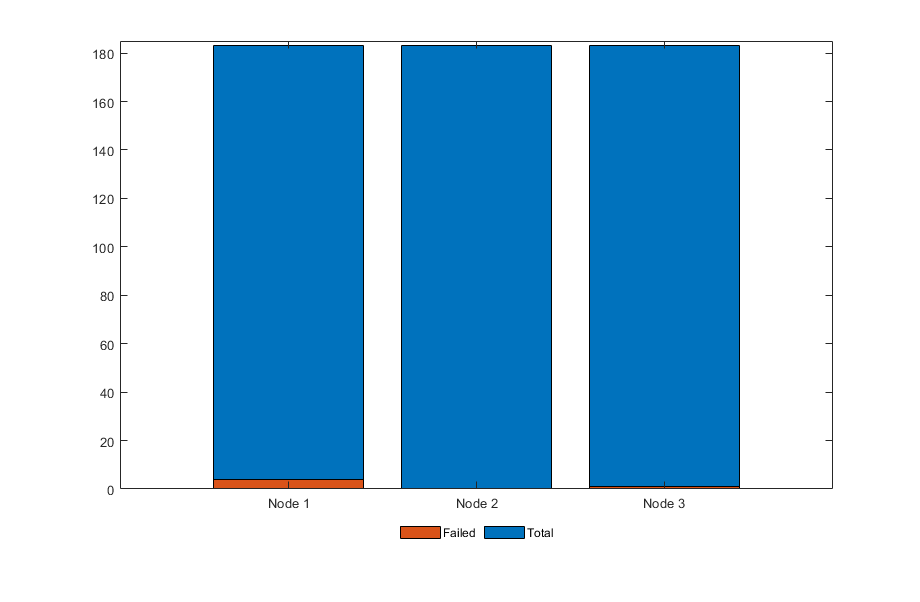
\includegraphics[width=0.8\textwidth]{research/network-communication-1h}
    \caption{\label{img:network-communication-1h}Wykres słupkowy przedstawiający wyniki 1-godzinnego testu komunikacji
        sieci}
\end{figure}

\FloatBarrier
\section{\label{sect:spectral-analisys}Analiza widmowa transmisji w~standardzie LoRa} Aby dokładniej zapoznać się z~tym,
jak działa komunikacja w~standardzie LoRa, wykonana została analiza widmowa transmisji pomiędzy modułami sieci.
Wykorzystane tutaj zostało narzędzie pozwalające na badanie fal radiowych bazujące na SDR (ang. \textsl{Software Defined
    Radio}) -- Hack RF One oraz darmowe, udostępnione w~domenie publicznej, oprogramowanie \textsl{gqrx} na platformę Linux.
Celem tego badania była obserwacja spektrum sygnałów radiowych w~okolicach częstotliwości, na jakich operuje LoRa, oraz
próba zaobserwowania czy możliwe jest metodą tą zobaczenie pojedynczych chirpów podczas transmisji. Stanowisko testowe
zostało wykorzystane także do zebrania zestawu próbek I/Q, które, w~późniejszym czasie, zostały poddane analizie
wykorzystując do tego środowisko MATLAB.

\subsection{\label{sect:spectral-in-gqrx}Obserwacje transmisji w~oprogramowaniu \textsl{gqrx}} Moduły zostały ustawione
na stanowisku testowym, odległość pomiędzy nimi podczas badania wynosiła, podobnie jak w~przypadku badania komunikacji,
około 0.45 m. W~odległości około 1~m od ustawionej sieci znajdowała się antena podłączona do Hack RF One. Oprogramowanie
\textsl{gqrx} ustawione zostało w~taki sposób, aby móc odczytywać w~nim dane zbierane przez urządzenie -- rozmiar okna
FFT na 1048576 próbek (maksymalna wartość dostępna w~programie), co dawało rozdzielczość pasma przenoszenia 1~Hz oraz
częstotliwość odświeżania na 60fps (ang. \textsl{frames per second} -- klatek na sekundę, maksymalna dostępna). Na tak
przygotowanym stanowisku testowym uruchomione zostały moduły. Aby uzyskać lepszą dokładność obserwacji, na modułach
wyłączona została funkcjonalność pracy na zegarze, a~transmisja uruchamiana była każdorazowo ręcznie (wykorzystując
przycisk na module MASTER).

Pierwsze próby obserwacji komunikacji przeprowadzone zostały na podstawowych ustawieniach modułów -- najniższa wartość
Spreading Factor, SF7 (7 bitów na symbol), pasmo 125kHz, radio coding rate, CR, 4/5. Takie parametry pozwalają sieci na
szybką komunikację, jednakże w~przypadku analizy widmowej nie pozwoliły one na dobrą obserwację transmisji. W~tym celu
parametr Spreading Factor przestawiony został na wartość maksymalną, SF12 (12 bitów na symbol). Spowodowało to
wydłużenie czasu każdej transmisji i~jednocześnie pozwoliło na lepszą obserwację. Korzystając ze zmodyfikowanych
parametrów, wykonane zostało kilkanaście transmisji i~w tym czasie obserwowane było, jak wygląda ich widmo. Rys.
\ref{img:waterfall-full-mid-transmission} przedstawione zostało, jak wyglądała obserwowana transmisja (tutaj: pełna sieć,
w~trakcie transmisji przez jeden z~modułów).

\begin{figure}[!htbp]
    \centering
    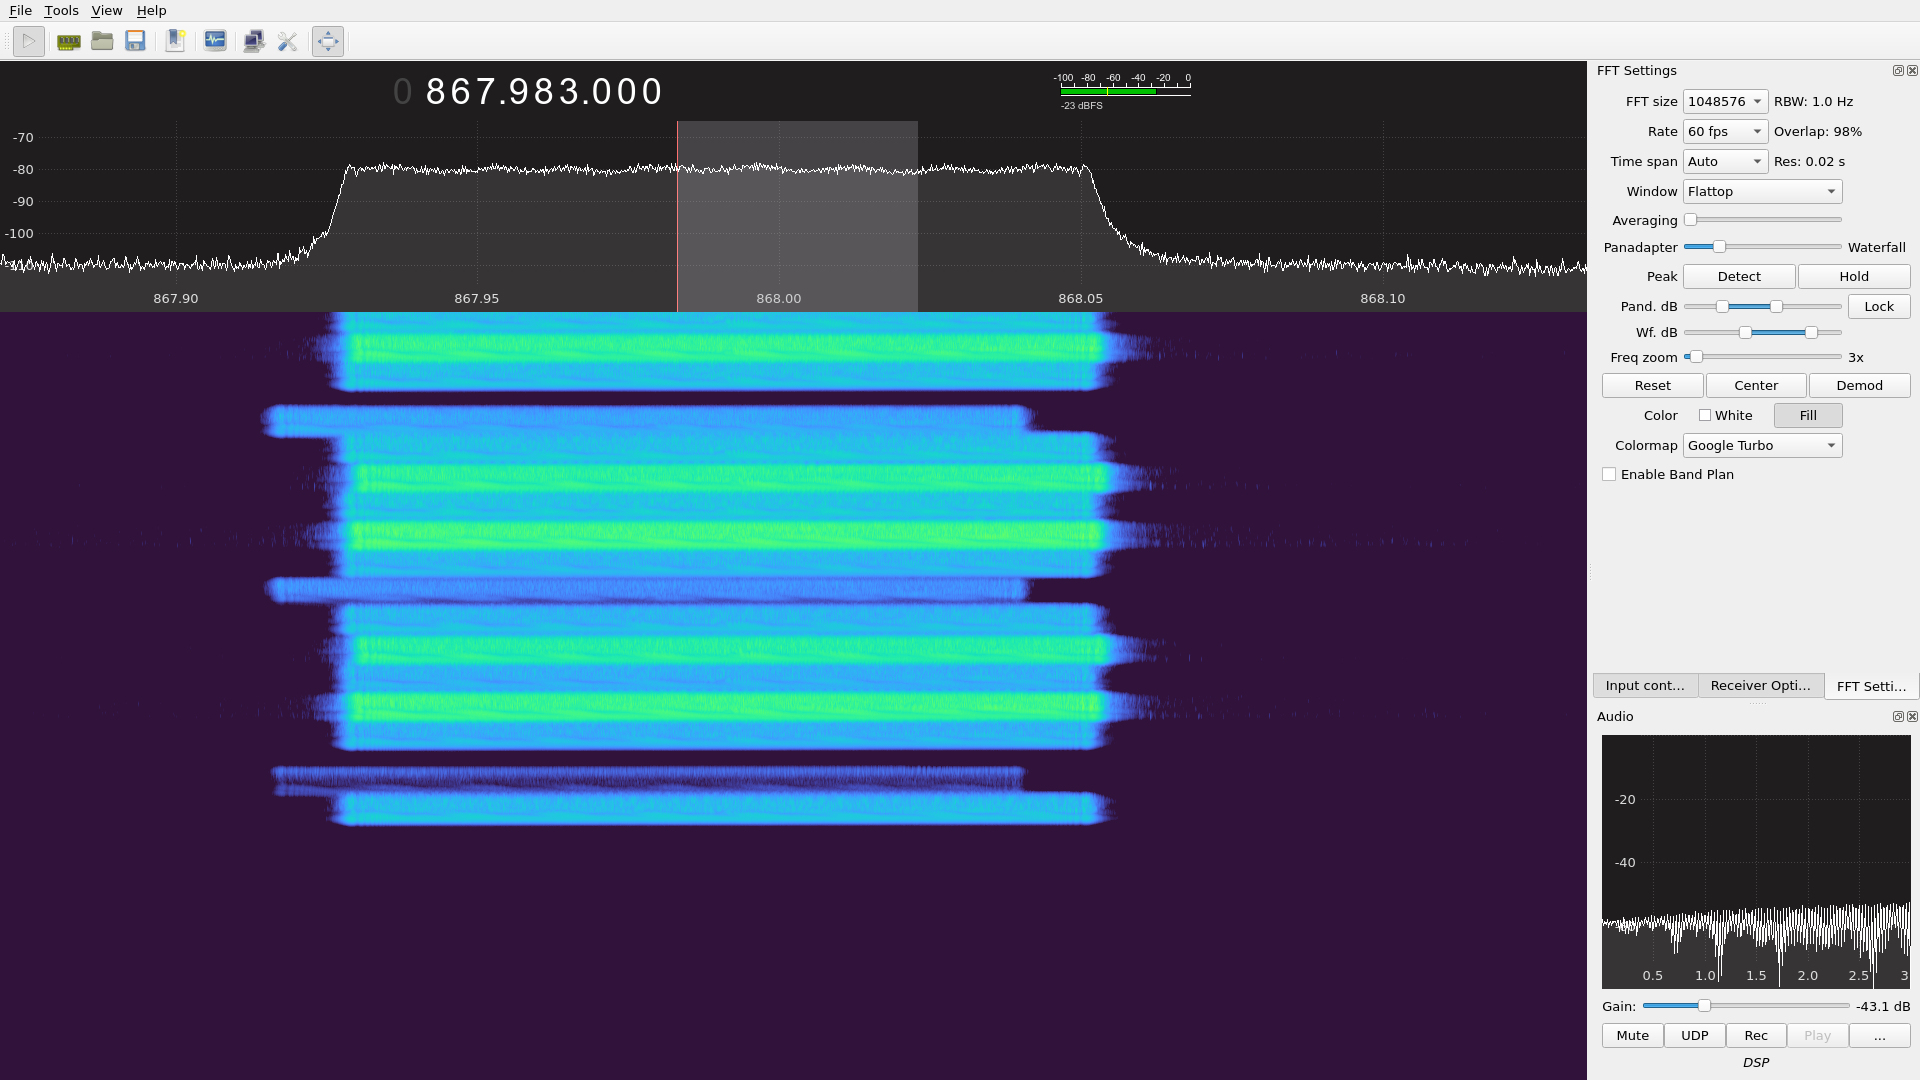
\includegraphics[width=0.9\textwidth]{research/waterfall-full-mid-transmission}
    \caption{\label{img:waterfall-full-mid-transmission}Zrzut ekranu z~programu pokazujący obserwowane transmisje}
\end{figure}

\FloatBarrier
Podczas badania wykonane zostały transmisje w~kilku konfiguracjach -- pełna sieć, 2~moduły SLAVE oraz 1~moduł SLAVE.
W~tym czasie wykonywane zostały zrzuty ekranów widoku z~programu \textsl{gqrx}. Na rys.
\ref{img:waterfall-full-no-timeouts}, \ref{img:waterfall-full-with-timeouts}, \ref{img:waterfall-one-slave} oraz
\ref{img:waterfall-two-slave} przestawione zostały wyniki obserwacji.

\begin{figure}[!htbp]
    \centering
    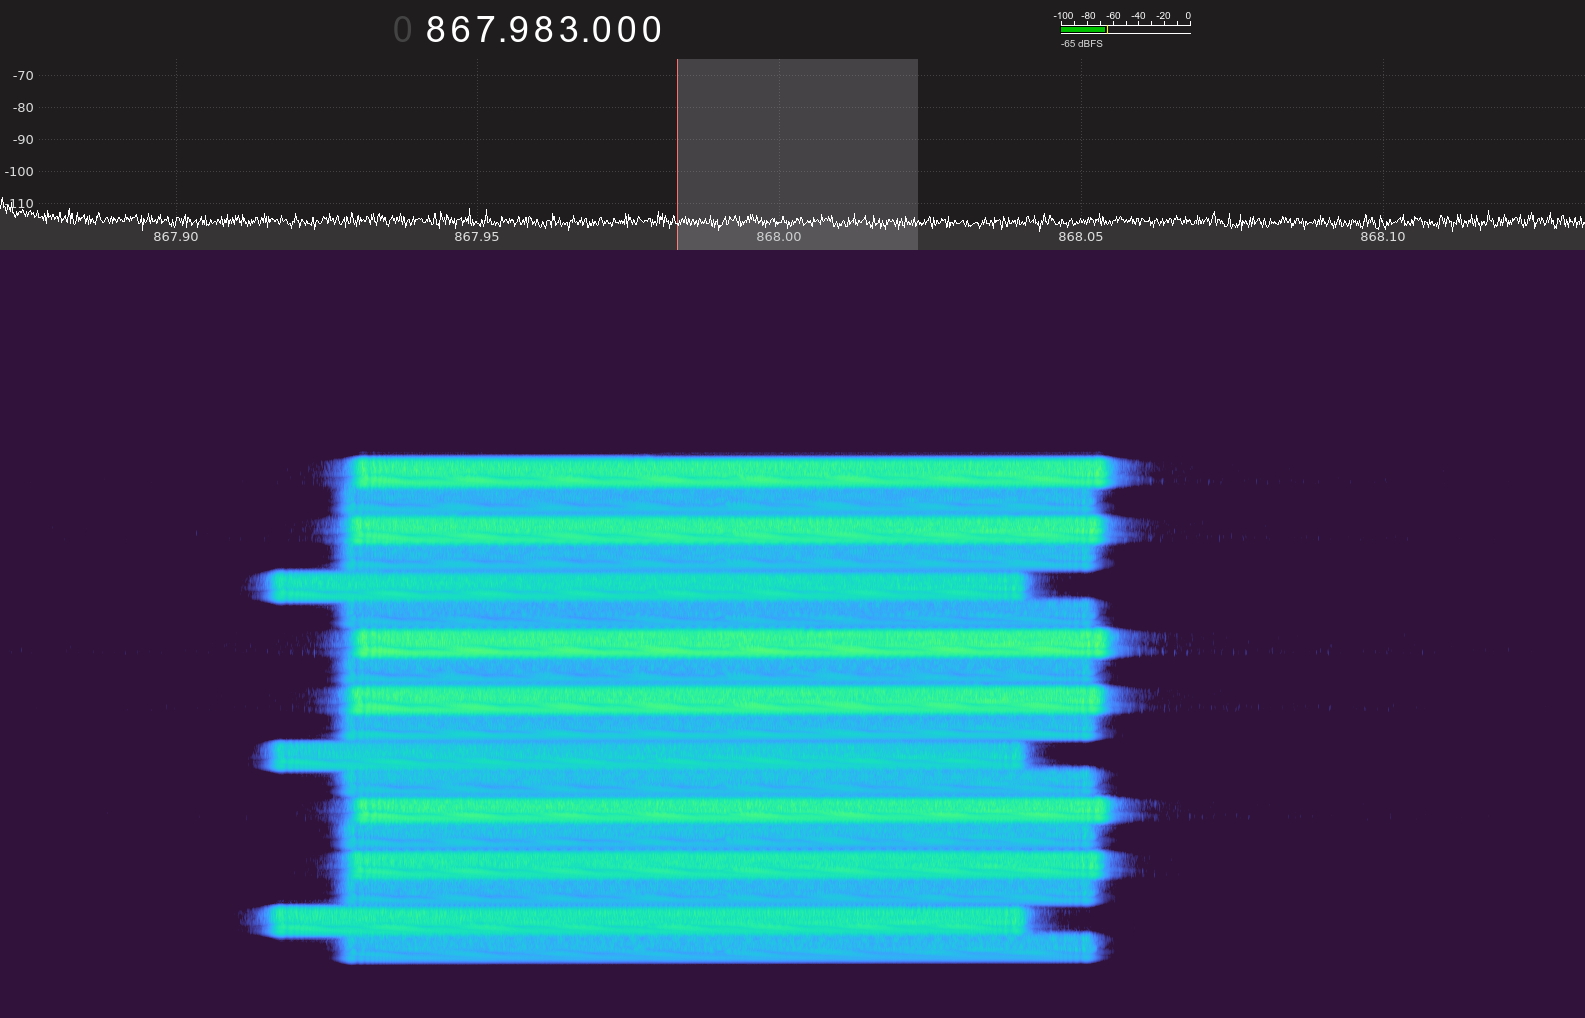
\includegraphics[width=0.9\textwidth]{research/waterfall-full-network-no-timeouts}
    \caption{\label{img:waterfall-full-no-timeouts}Widok na komunikację pełnej sieci, bez wystąpienia problemów
        z~komunikacją}
\end{figure}

\begin{figure}[!htbp]
    \centering
    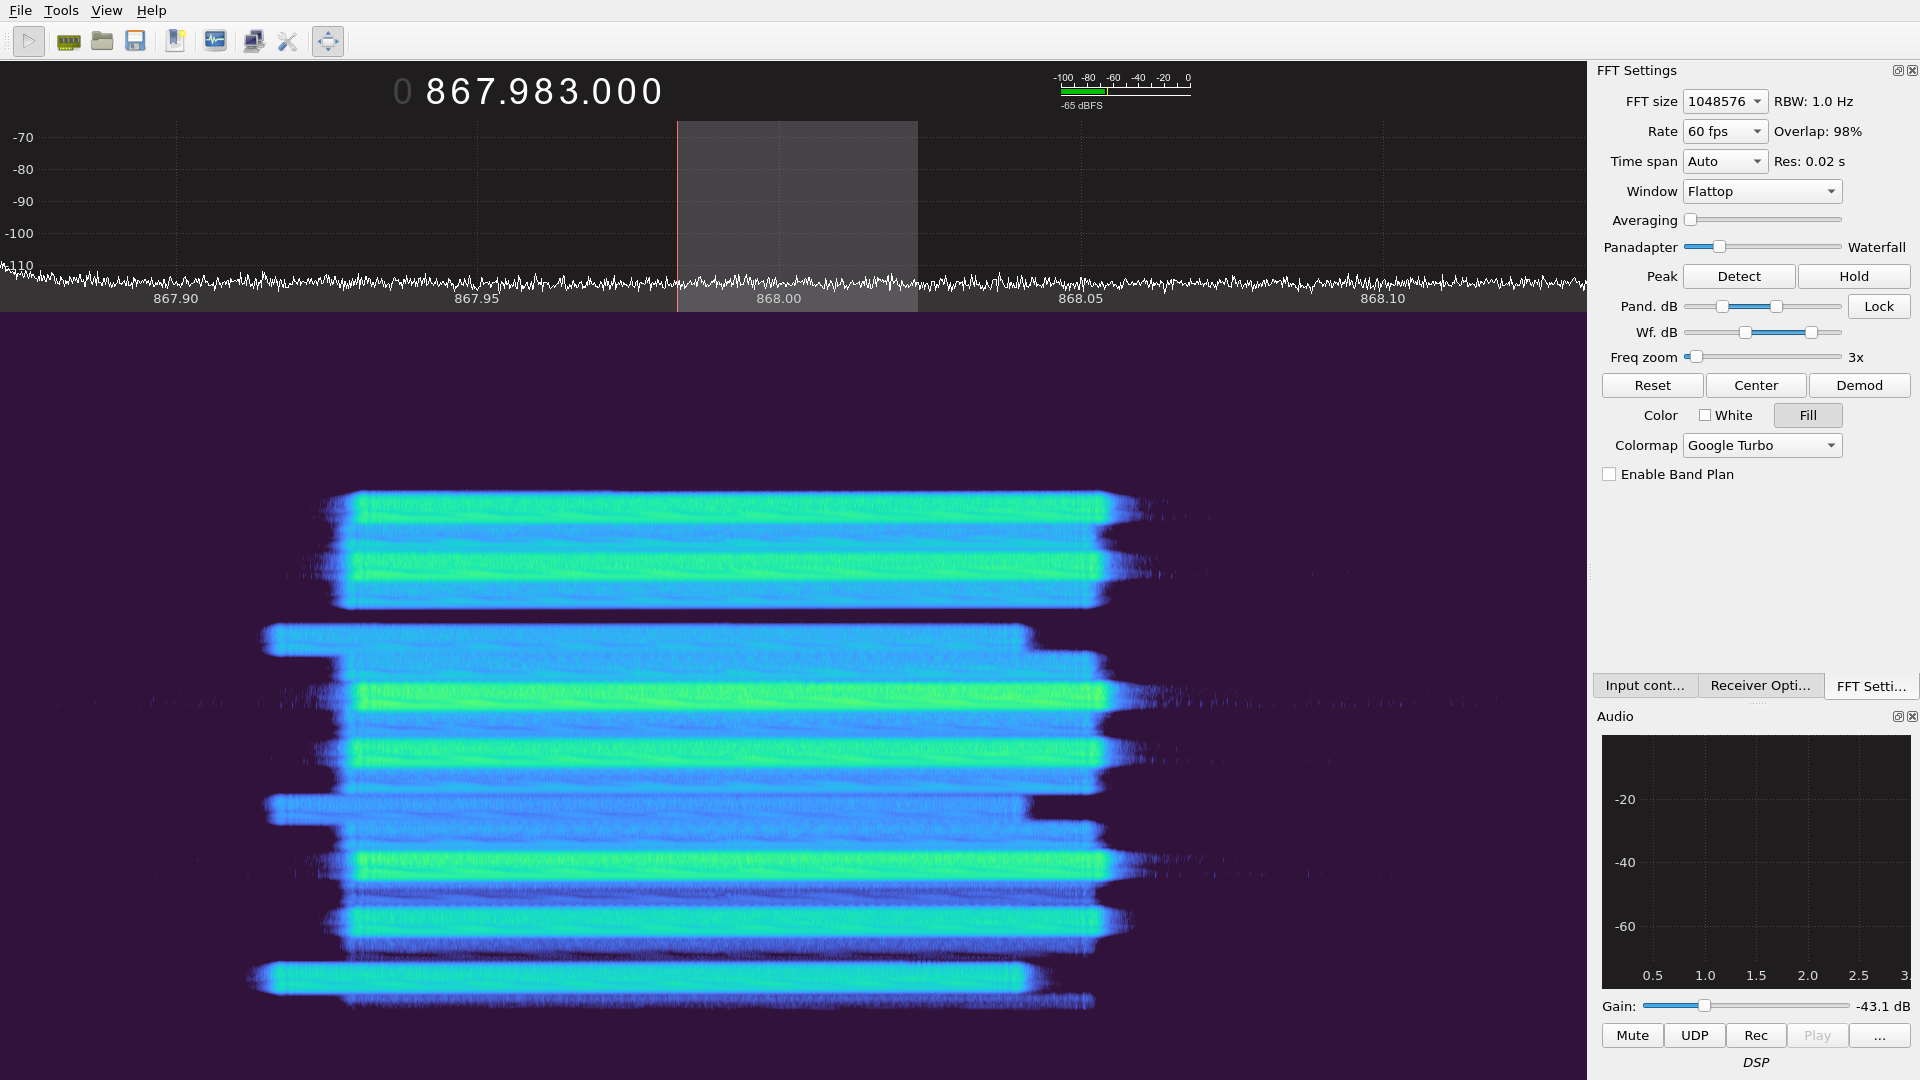
\includegraphics[width=0.9\textwidth]{research/waterfall-full-network-with-timeouts}
    \caption{\label{img:waterfall-full-with-timeouts}Widok na komunikację pełnej sieci, z~widocznymi przerwami, gdy
        jeden z~modułów nie odpowiedział na zapytanie}
\end{figure}

\begin{figure}[!htbp]
    \centering
    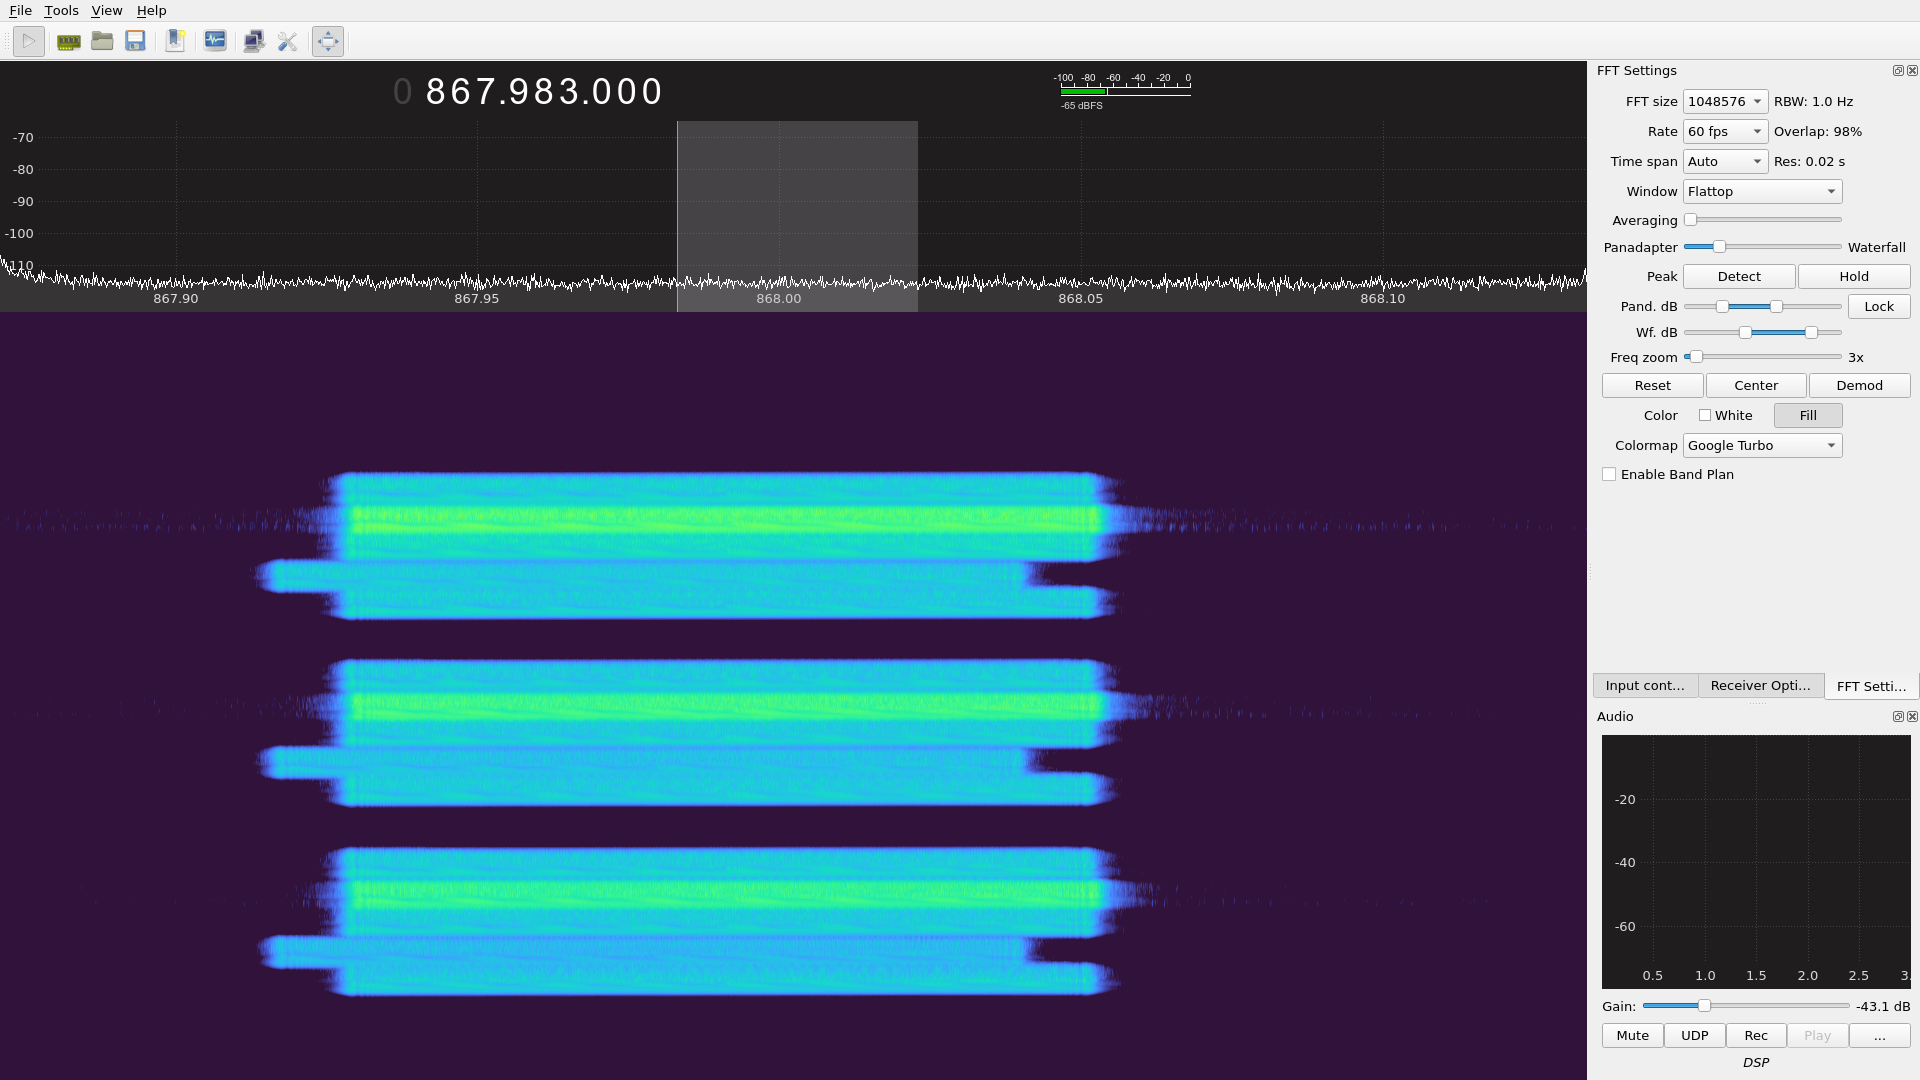
\includegraphics[width=0.9\textwidth]{research/waterfall-two-slave-network}
    \caption{\label{img:waterfall-one-slave}Widok na komunikację w~sieci dwoma modułami SLAVE włączonymi, a~jednym
        wyłączonym}
\end{figure}

\begin{figure}[!htbp]
    \centering
    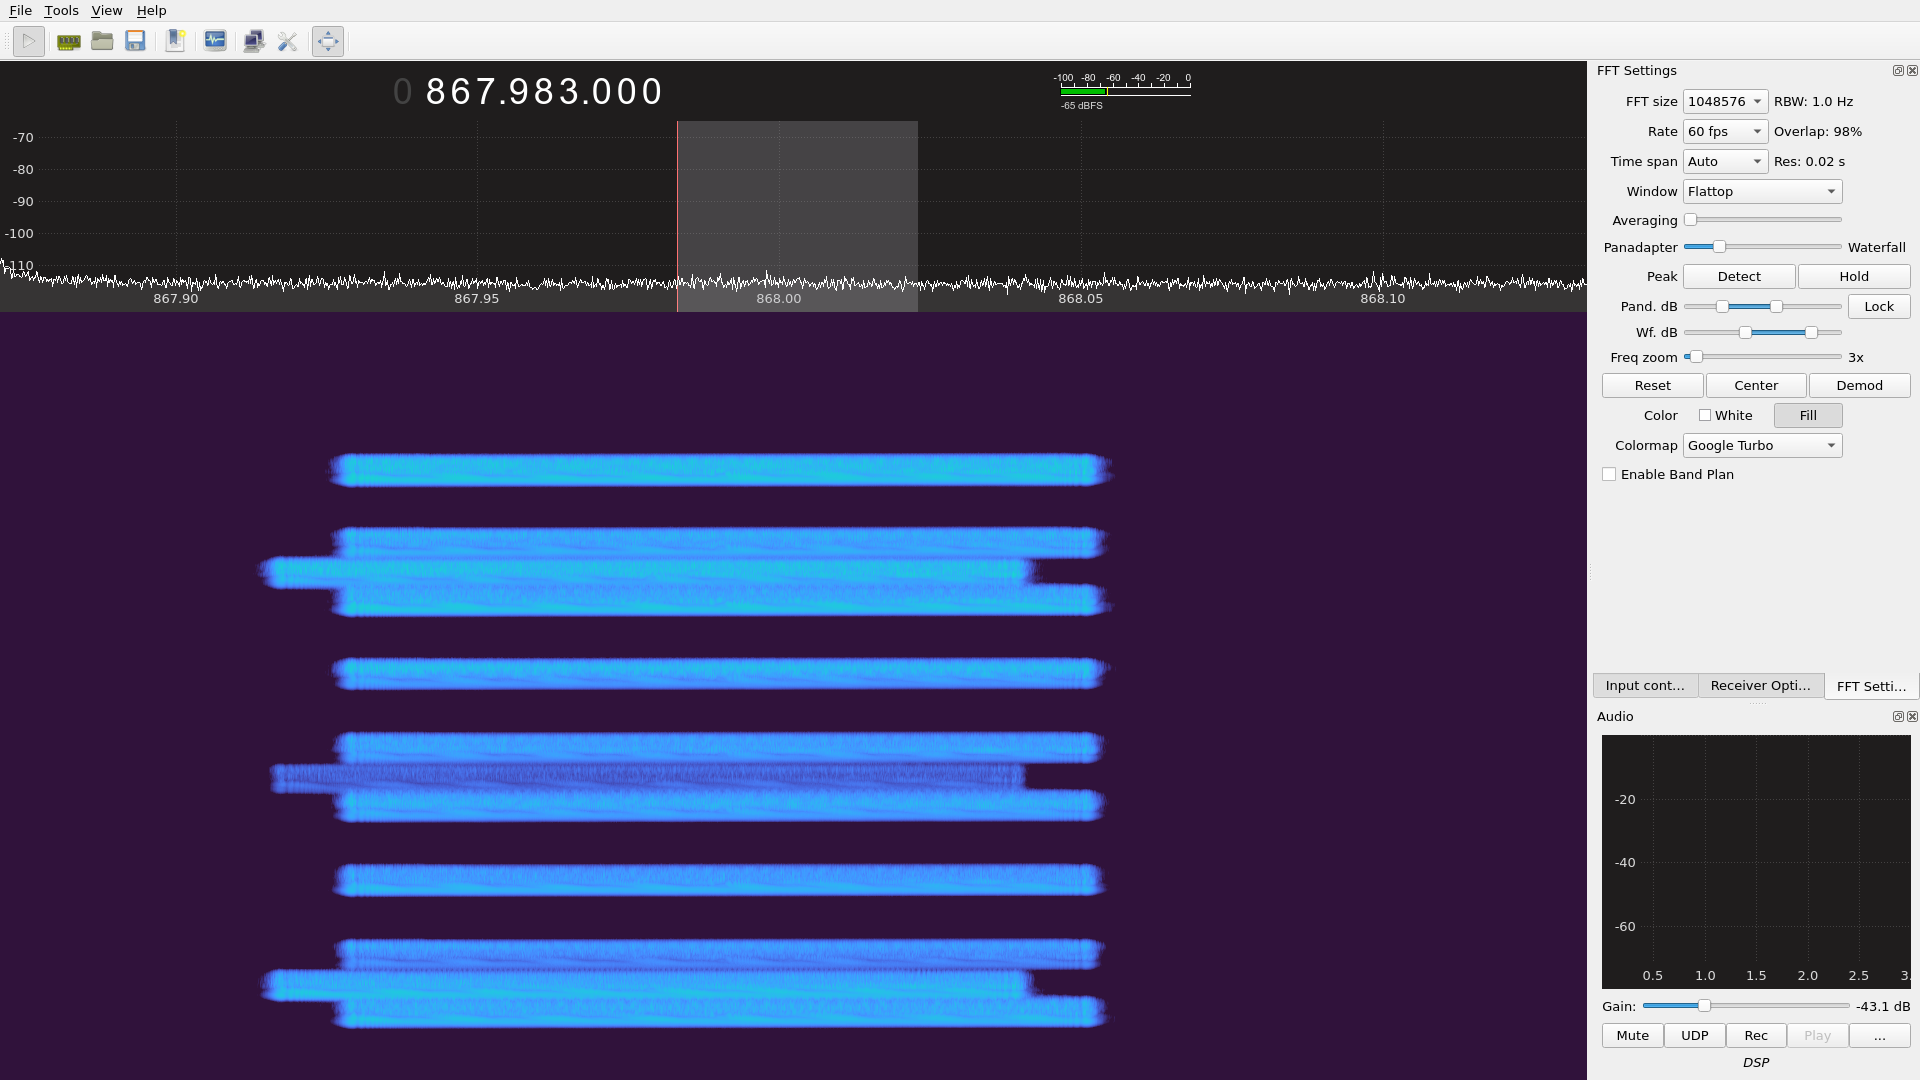
\includegraphics[width=0.9\textwidth]{research/waterfall-one-slave-network}
    \caption{\label{img:waterfall-two-slave}Widok na komunikację w~sieci z~tylko jednym modułem SLAVE włączonymi}
\end{figure}

\FloatBarrier
W~przypadku, gdzie udało się zaobserwować pełną komunikację, gdzie nie wystąpiły żadne problemy, wyraźnie widać 9~wymian
pomiędzy modułami (18 transmisji). Natomiast w~przypadkach, gdy pojawił się błąd, bądź dany moduł był wyłączony wyraźnie
widać to w~zaobserwowanym zapisie. Niestety w~przypadku obserwacji wykorzystując do tego program \textsl{gqrx} nie udało
zaobserwować się pojedynczych elementów każdej transmisji (pojedynczych chirpów, preambuły czy wysyłanych symboli). Jest
to związane z~ograniczeniami oprogramowania co do maksymalnej szybkości odświeżania widoku na ekranie.

Poza obserwacją tzw. wykresów wodospadowych (pokazujących zmiany w~widmie w~czasie) udało się także zebrać zapisy
rozkładu częstotliwości sygnałów podczas transmisji wykonywanych przez moduły. Przedstawione zostało to na rys.
\ref{img:frequency-graph-no-transmission}, \ref{img:frequency-graph-master-request} oraz
\ref{img:frequency-graph-slave-response}. Ciekawym faktem jest tutaj widoczna w~przypadku transmisji z~modułów SLAVE
wyższa moc sygnałów. Spowodowane to było najprawdopodobniej faktem, że były umieszczone bliżej anteny podłączonej do
urządzenia zbierającego dane.

\begin{figure}[!htbp]
    \centering
    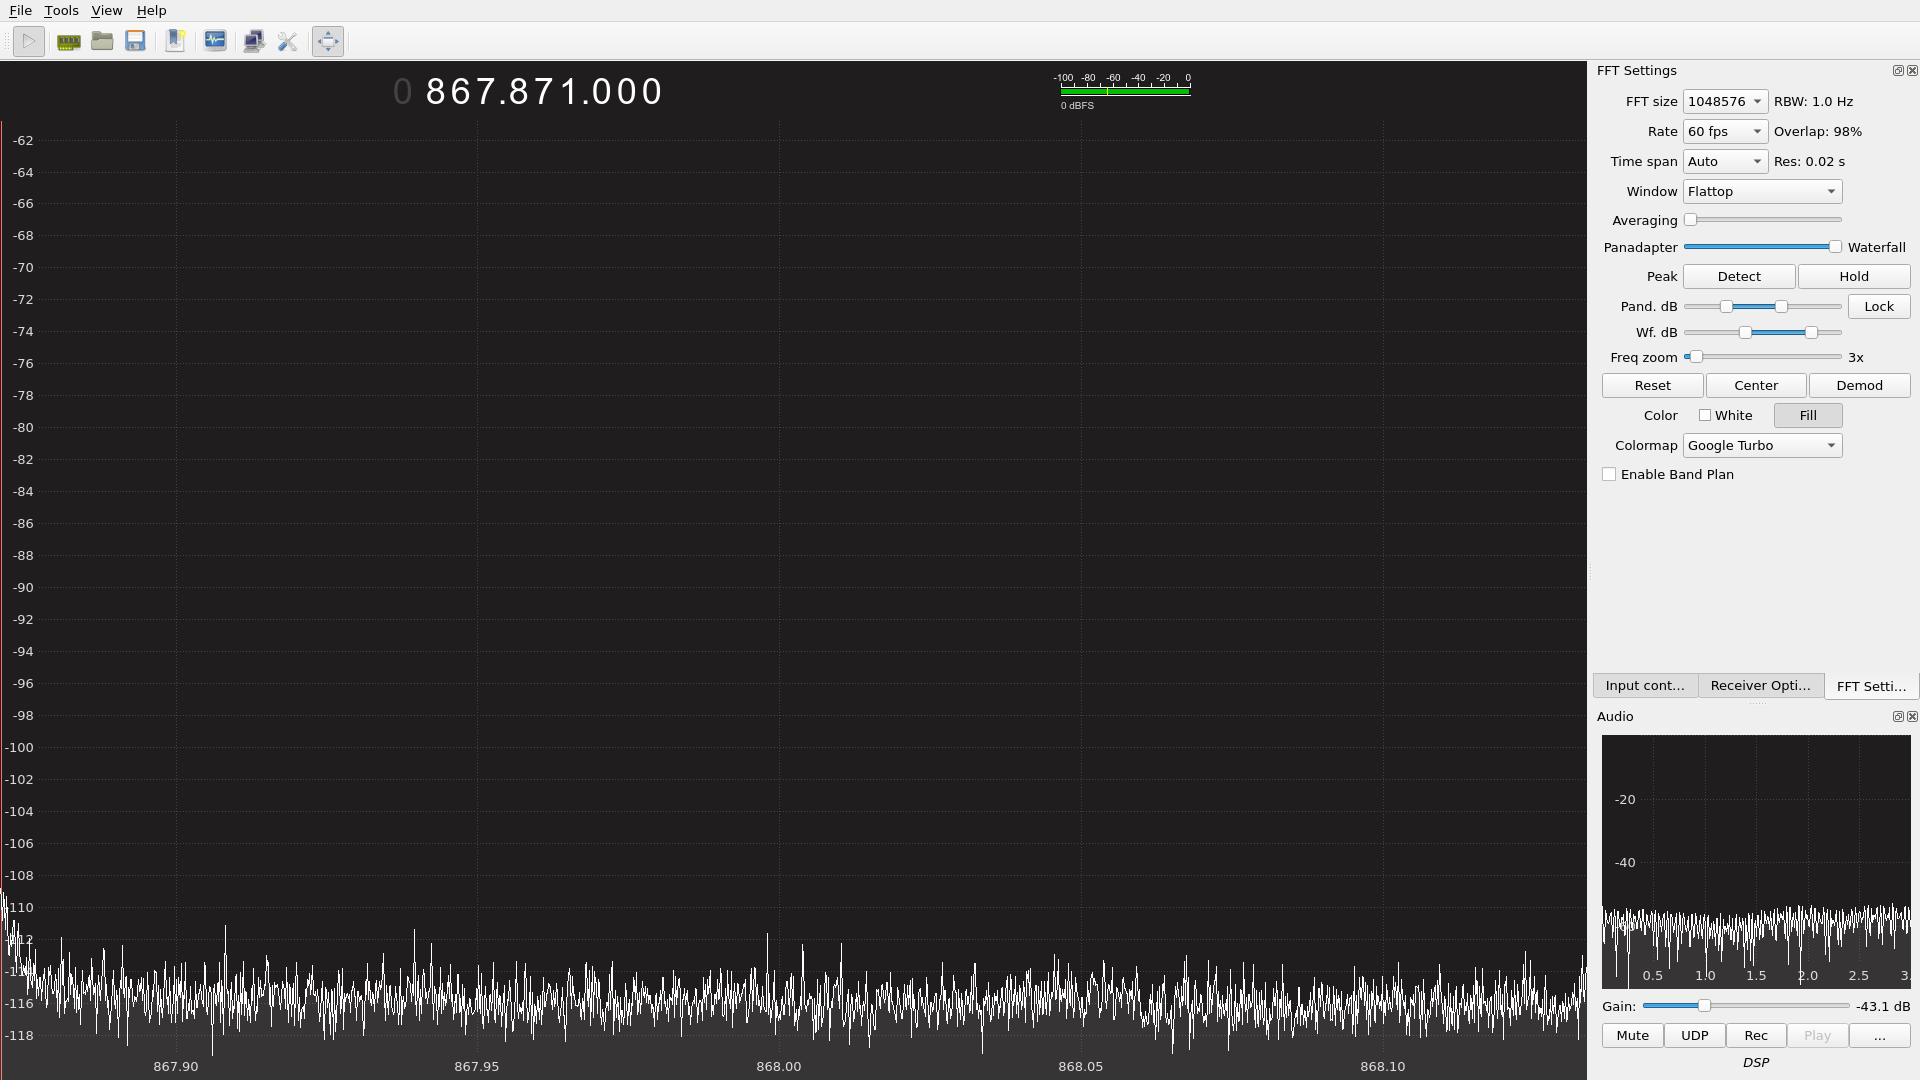
\includegraphics[width=0.9\textwidth]{research/frequency-graph-no-transmission}
    \caption{\label{img:frequency-graph-no-transmission}Widok spektrum częstotliwości, gdy żaden z~modułów nie transmituje}
\end{figure}

\begin{figure}[!htbp]
    \centering
    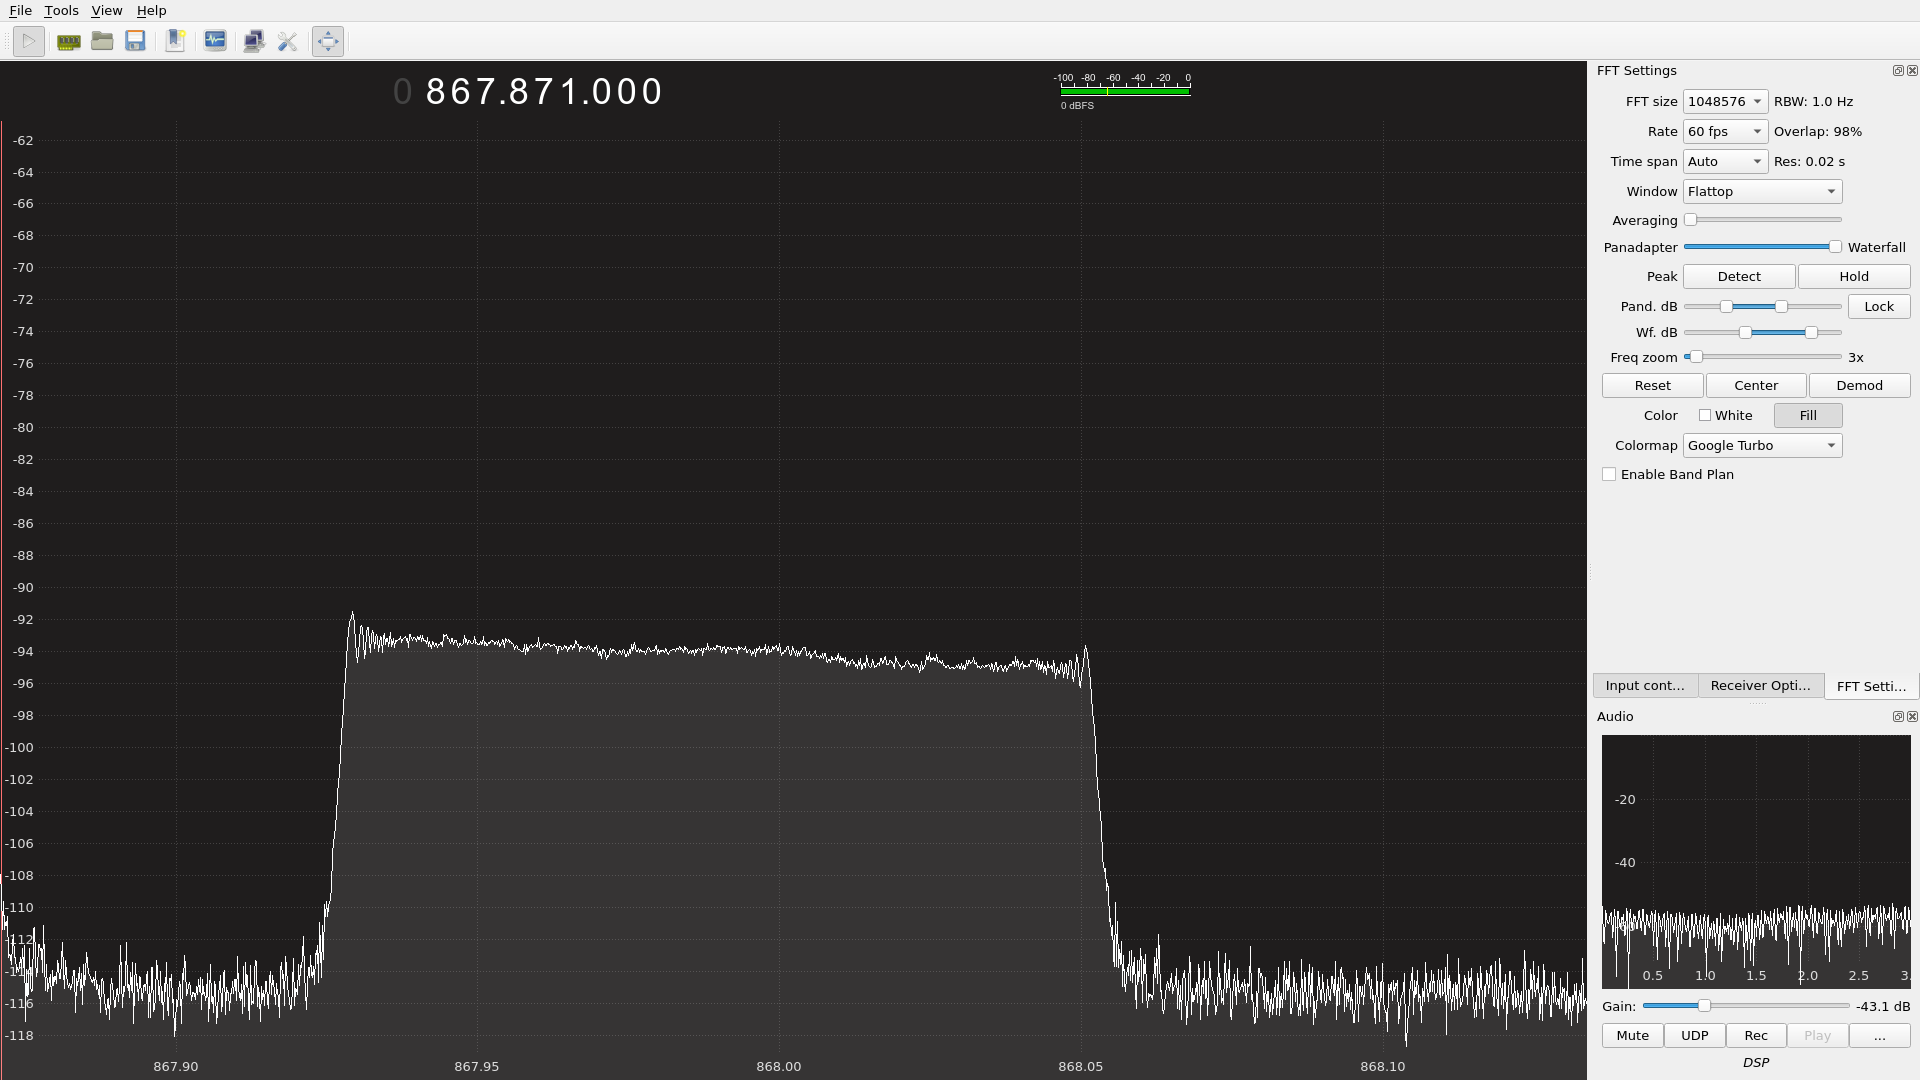
\includegraphics[width=0.9\textwidth]{research/frequency-graph-master-request}
    \caption{\label{img:frequency-graph-master-request}Widok spektrum częstotliwości podczas transmisji modułu MASTER}
\end{figure}

\begin{figure}[!htbp]
    \centering
    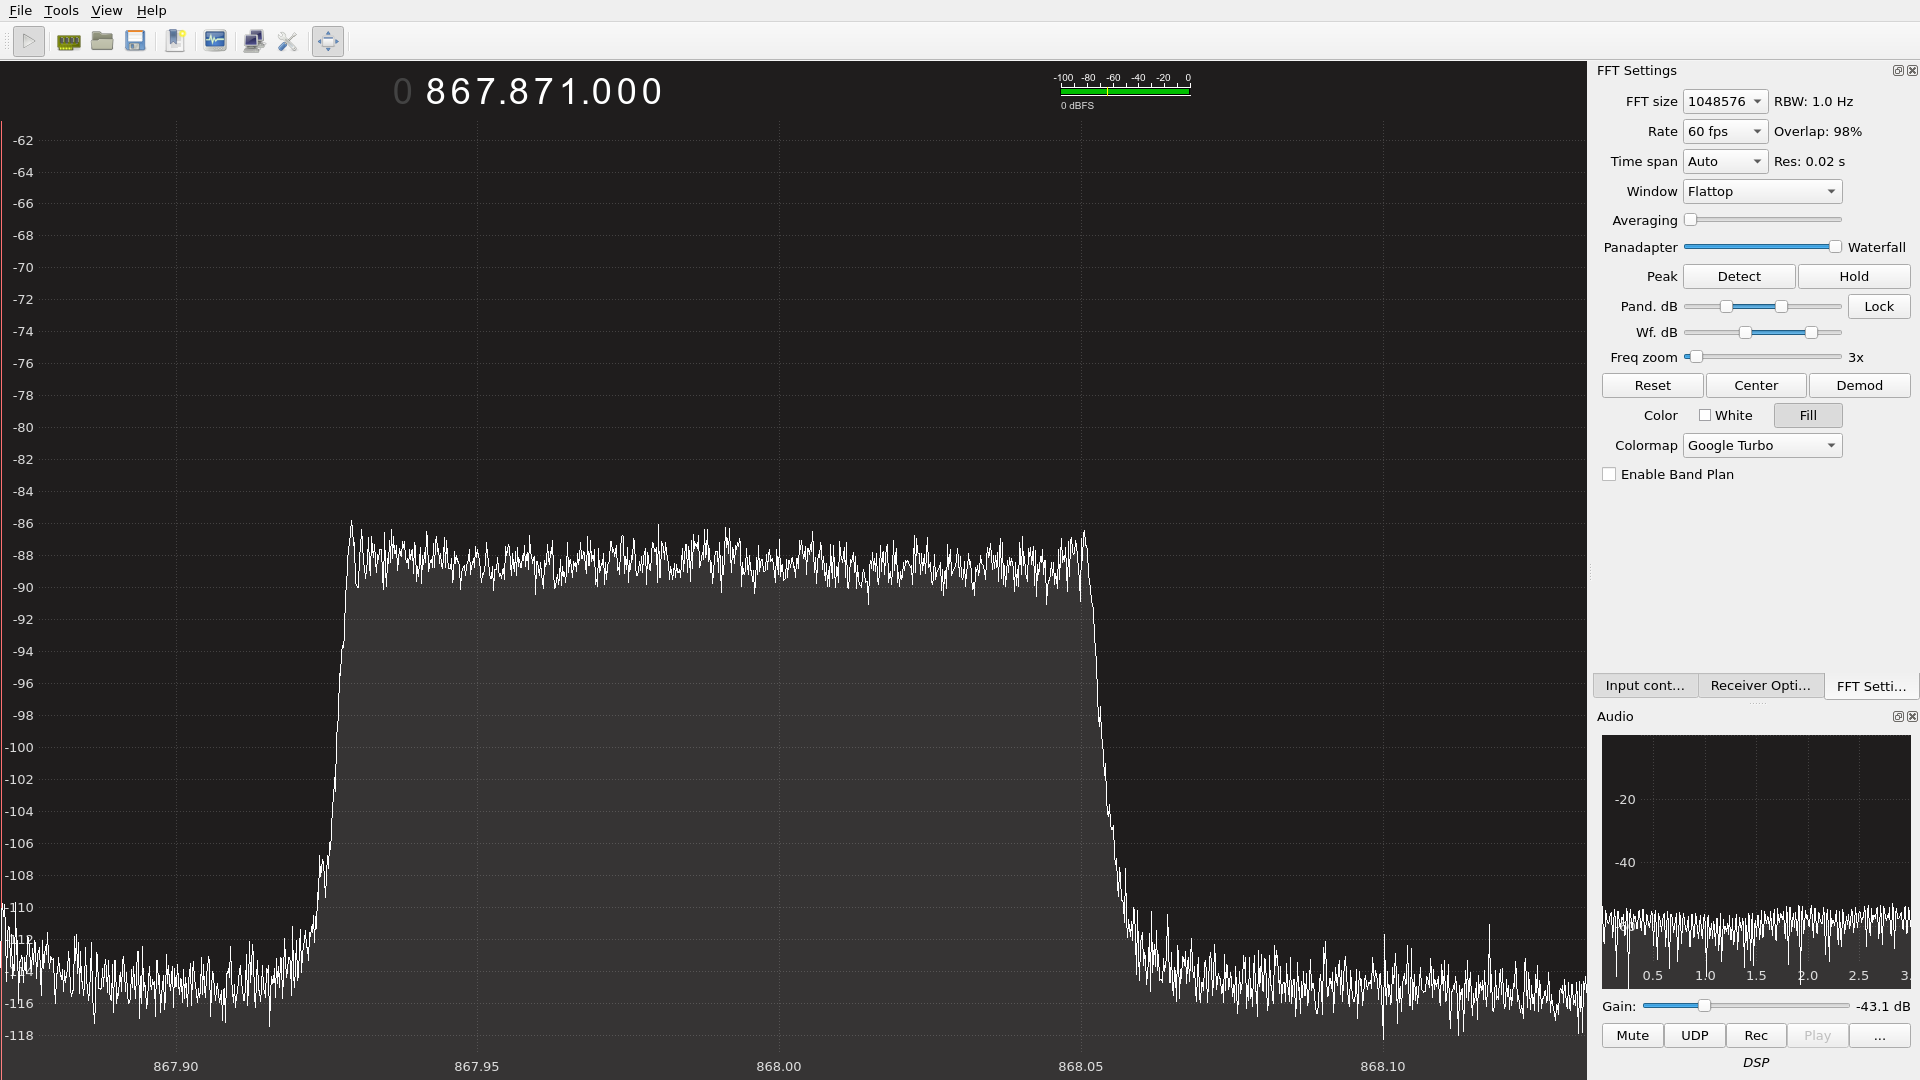
\includegraphics[width=0.9\textwidth]{research/frequency-graph-slave-response}
    \caption{\label{img:frequency-graph-slave-response}Widok spektrum częstotliwości podczas transmisji modułów SLAVE}
\end{figure}

\FloatBarrier
\subsection{\label{sect:iq-data-gqrx}Analiza zapisów danych I/Q zebranych \textsl{gqrx}} Ponieważ wykresy obserwowane
bezpośrednio w~oprogramowaniu \textsl{gqrx} nie pozwalały na analizę przesyłanych transmisji z~modułów, wykorzystana
została funkcja zapisu rejestrowanych danych do postaci I/Q (ang. \textsl{In-phase and quadrature components}) do plików
RAW. W~celu późniejszej analizy danych wykonane zostały 3~zapisy pełnych wymian danych w~sieci w~różnych konfiguracjach,
z~parametrami modułów ustawionych na podstawowych wartościach z~wyjątkiem Spreading Factor. Parametr ten ustawiony
został na wartość maksymalną (SF12, 12 bitów na symbol), tak aby uzyskać najlepsze szanse na analizę transmisji.

Dane I/Q to metoda opisu wielkości i~danych fazowych rejestrowanego sygnału, gdzie falę sinusoidalną można przedstawić
w~formie współrzędnych biegunowych \cite{ni-iq-data} korzystając z~równania:
\begin{equation}
    f(t) = A\cos{2\pi{ft}+\varphi}
\end{equation}
Zarejestrowane w~ten sposób dane (sinusoidę z~modulacją) można rozłożyć na dwie sinusoidy z~modulacją amplitudy, które
przesunięte są względem siebie w~fazie o ${\pi}/2$ radianów (90 stopni). Zarejestrowaną falę można wówczas przedstawić
w~złożonym układzie współrzędnych kartezjańskich, w~postaci składowych rzeczywistej i~urojonej, korzystając z~równań:
\begin{equation}
    I(t) = A\cos{\varphi}\cos{2\pi{ft}} \quad\text{(Składowa rzeczywista)}
\end{equation}
\begin{equation}
    Q(t) = A\sin{\varphi}\sin{2\pi{ft}} \quad\text{(Składowa urojona)}
\end{equation}

Korzystając z~zarejestrowanych zapisów, gdzie każdy miał długość około 25 sekund i~składał się z~około 25 milionów
próbek (związane z~ustawionym oknem FFT, milion próbek na sekundę) wykonana została ich analiza w~środowisku MATLAB.
Napisana została funkcja pozwalająca na generowanie spektrogramów pełnego zarejestrowanego sygnału oraz spektrogramów
zbliżenia na konkretne, wyznaczone, elementy. Kod źródłowy przedstawiony został na listingach
\ref{lst:matlab-spectrogram-zoom-1}, \ref{lst:matlab-spectrogram-zoom-2} oraz \ref{lst:matlab-spectrogram-zoom-3}
(przedstawiają kolejno: argumenty wejściowe funkcji, właściwe generowanie spektrogramów oraz funkcje pomocnicze do
ładowania danych z~plików RAW i~eksportu wygenerowanych wykresów).

\lstinputlisting[
    language=matlab,
    linerange={3-12},
    caption={Funkcja do analizy danych I/Q w~MATLAB -- argumenty wejściowe},
    label={lst:matlab-spectrogram-zoom-1},
    float=htbp
]{gqrx-spectrograms/spectrogramzoom.m}

\lstinputlisting[
    language=matlab,
    linerange={14-40},
    caption={Funkcja do analizy danych I/Q w~MATLAB -- generowanie pełnego spektrogramu oraz zbliżenia na wycinek},
    label={lst:matlab-spectrogram-zoom-2},
    float=htbp
]{gqrx-spectrograms/spectrogramzoom.m}

\lstinputlisting[
    language=matlab,
    linerange={43-57},
    caption={Funkcja do analizy danych I/Q w~MATLAB -- funkcje pomocnicze},
    label={lst:matlab-spectrogram-zoom-3},
    float=htbp
]{gqrx-spectrograms/spectrogramzoom.m}

Argumentami wejściowymi funkcji są: plik wejściowy (zawierający dane I/Q), ścieżka oraz nazwa pliku, gdzie wygenerowany
wykres ma zostać zapisany, zasięg próbek, na jakim ma zostać wykonane zbliżenie oraz dodatkowe parametry do funkcji
\texttt{spectrogram} -- wielkość okna, częstotliwość próbkowania, liczba nakładających się próbek, liczba punktów do
dyskretnej transformaty Fouriera.

\FloatBarrier
Funkcja pomocnicza, wykorzystywana do ładowania plików RAW, bazuje na równianach opisujących składowe rzeczywistą
i~urojoną. Plik zostaje otwarty w~momencie wywołania funkcji, a~jego zawartość odczytana w~postaci 32-bitowych wartości
zmiennoprzecinkowych (float32) z~najbardziej znaczącym bajtem jako pierwszym (ang. \textsl{Big endian}). Następnie
zawartość pliku ładowana jest do pamięci programu, modyfikując je do postaci złożonej (ang. \textsl{Complex}).

Generowanie spektrogramów wykorzystuje wbudowaną funkcję \texttt{spectrogram}. W~przypadku generowania wykresu dla
całego sygnału wykorzystywane są tylko argumenty wejściowe. Dodatkowo na podstawie wprowadzonych wartości, gdzie ma
zostać wykonane zbliżenie, na wykresie rysowane są linie pionowe na osi X. Korzystając z~długości (wielkości) tablicy
danych wejściowych, ustalane są ilość oraz rozstawienie podziałki. Natomiast w~przypadku wykresu zbliżenia, pierwszym
elementem jest wyznaczenie zakresu próbek, na podstawie których wygenerowany ma zostać spektrogram. Korzystając z~tych
dodatkowych zmiennych oraz pozostałych argumentów wejściowych generowany jest spektrogram zbliżenia. Ostatnim krokiem
w~funkcji jest eksport wykresu do pliku. Wykorzystywana jest do tego zaimplementowana funkcja pomocnicza
\texttt{exportfigure}. Zdefiniowane w~niej zmienne wykorzystywane są do zachowania poprawnych proporcji, tak aby wykres
miał największą możliwą czytelność.

\FloatBarrier
Korzystając z~zaimplementowanej funkcji, wygenerowane zostały spektrogramy jednego z~zarejestrowanych sygnałów, stosując
zwiększające przybliżenie, w~celu uzyskania jak najlepszego widoku na pojedynczą transmisję. Wygenerowane wykresy
przedstawione zostały przedstawione na rys. \ref{img:signal1-level1}, \ref{img:signal1-level2}, \ref{img:signal1-level3}
oraz \ref{img:signal1-level4} (zbliżenia w~czasie 2.5 s~a 6~s, pokazujące 3~transmisje, do 3.6 s~a 4.6 s, pokazując
dokładniej 1~transmisję).

\begin{figure}[!htbp]
    \centering
    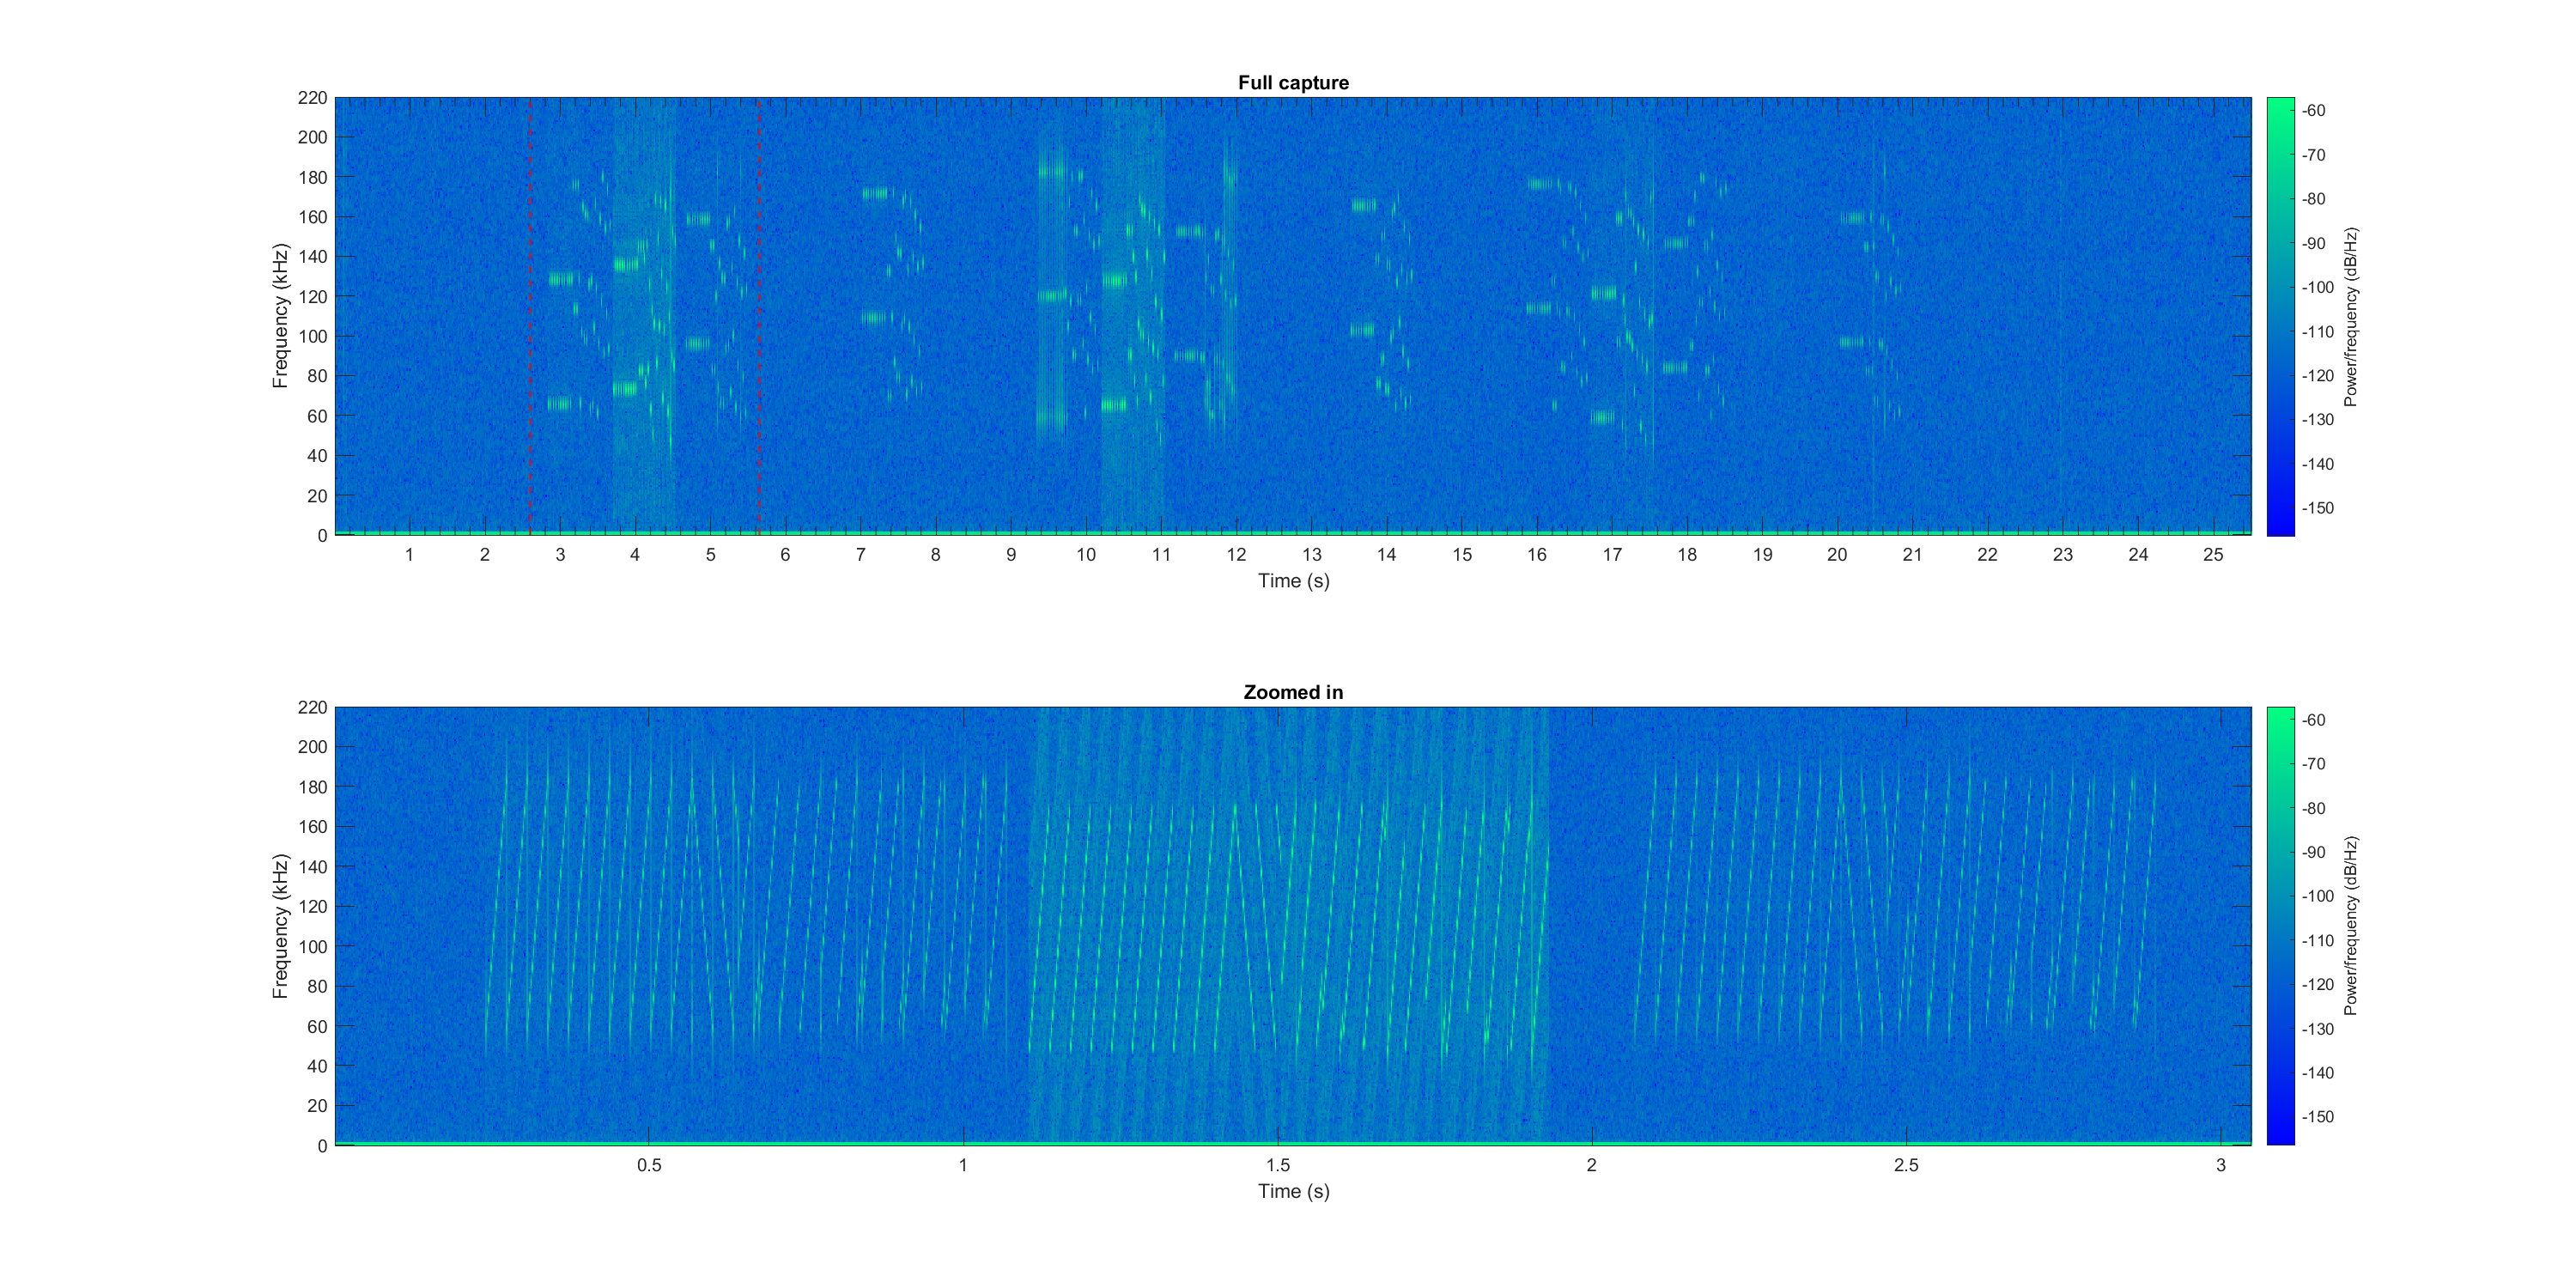
\includegraphics[width=\textwidth]{research/gqrx/zoom-win1024-sig1-lvl1}
    \caption{\label{img:signal1-level1}Spektrogram sygnałów z~pierwszej próbki wraz ze zbliżeniem między 2.5 s~a 5.5 s}
\end{figure}

\begin{figure}[!htbp]
    \centering
    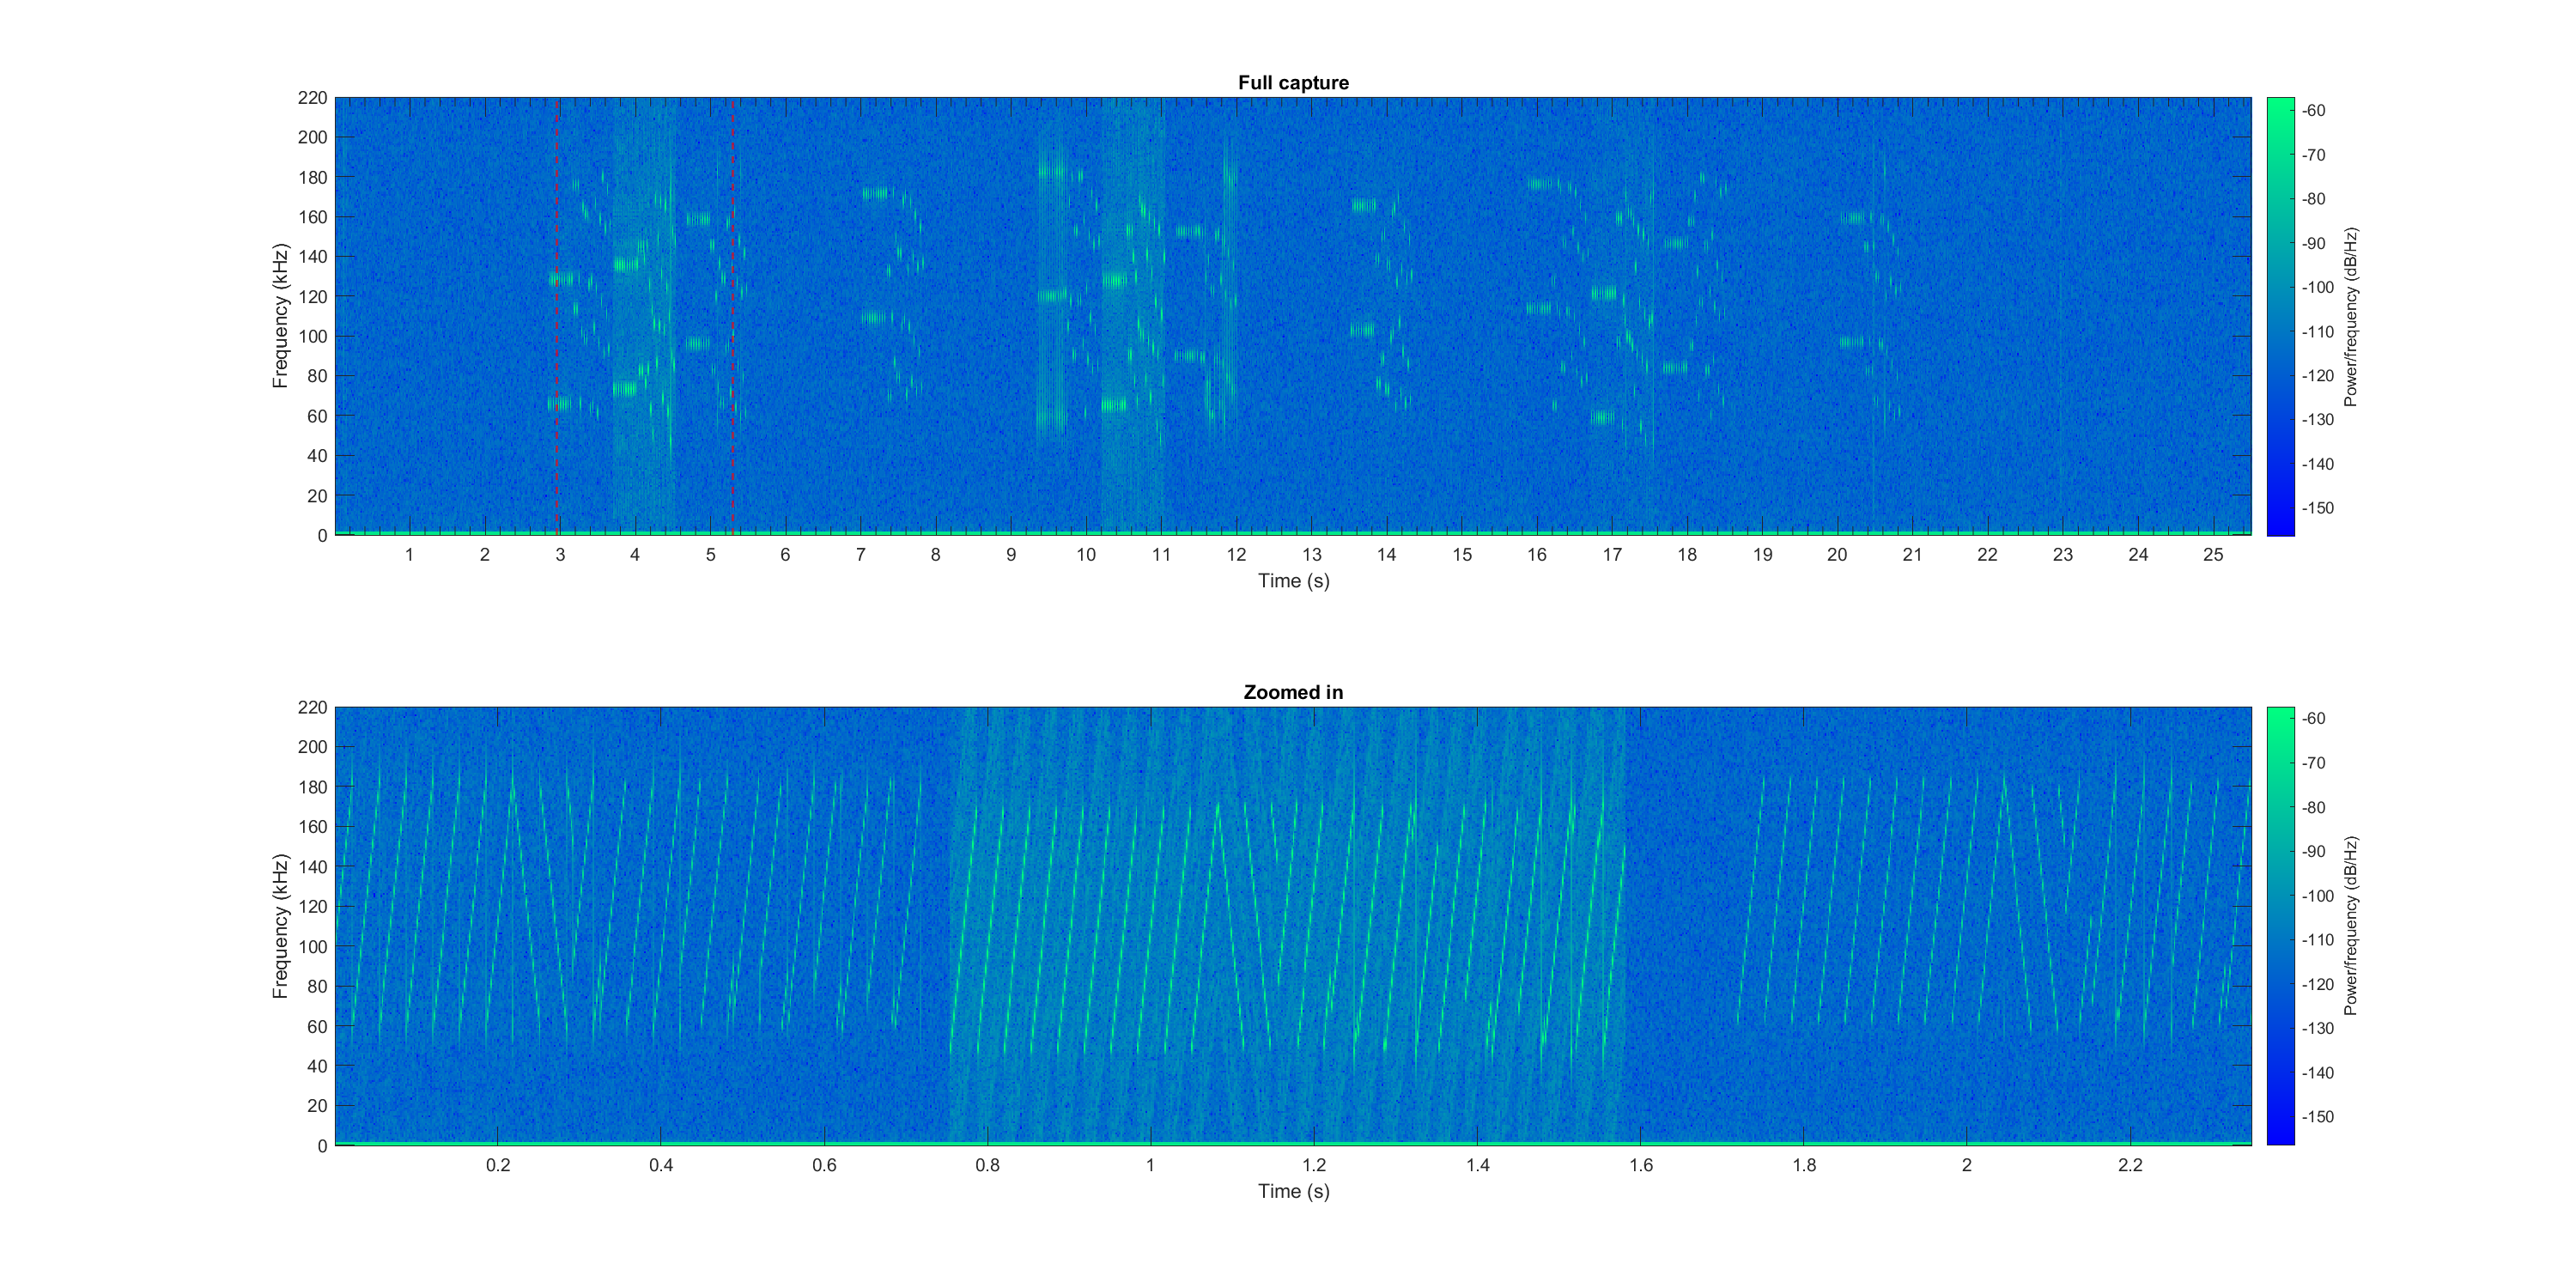
\includegraphics[width=\textwidth]{research/gqrx/zoom-win1024-sig1-lvl2}
    \caption{\label{img:signal1-level2}Spektrogram sygnałów z~pierwszej próbki wraz ze zbliżeniem między 3~s a 5.1 s}
\end{figure}

\begin{figure}[!htbp]
    \centering
    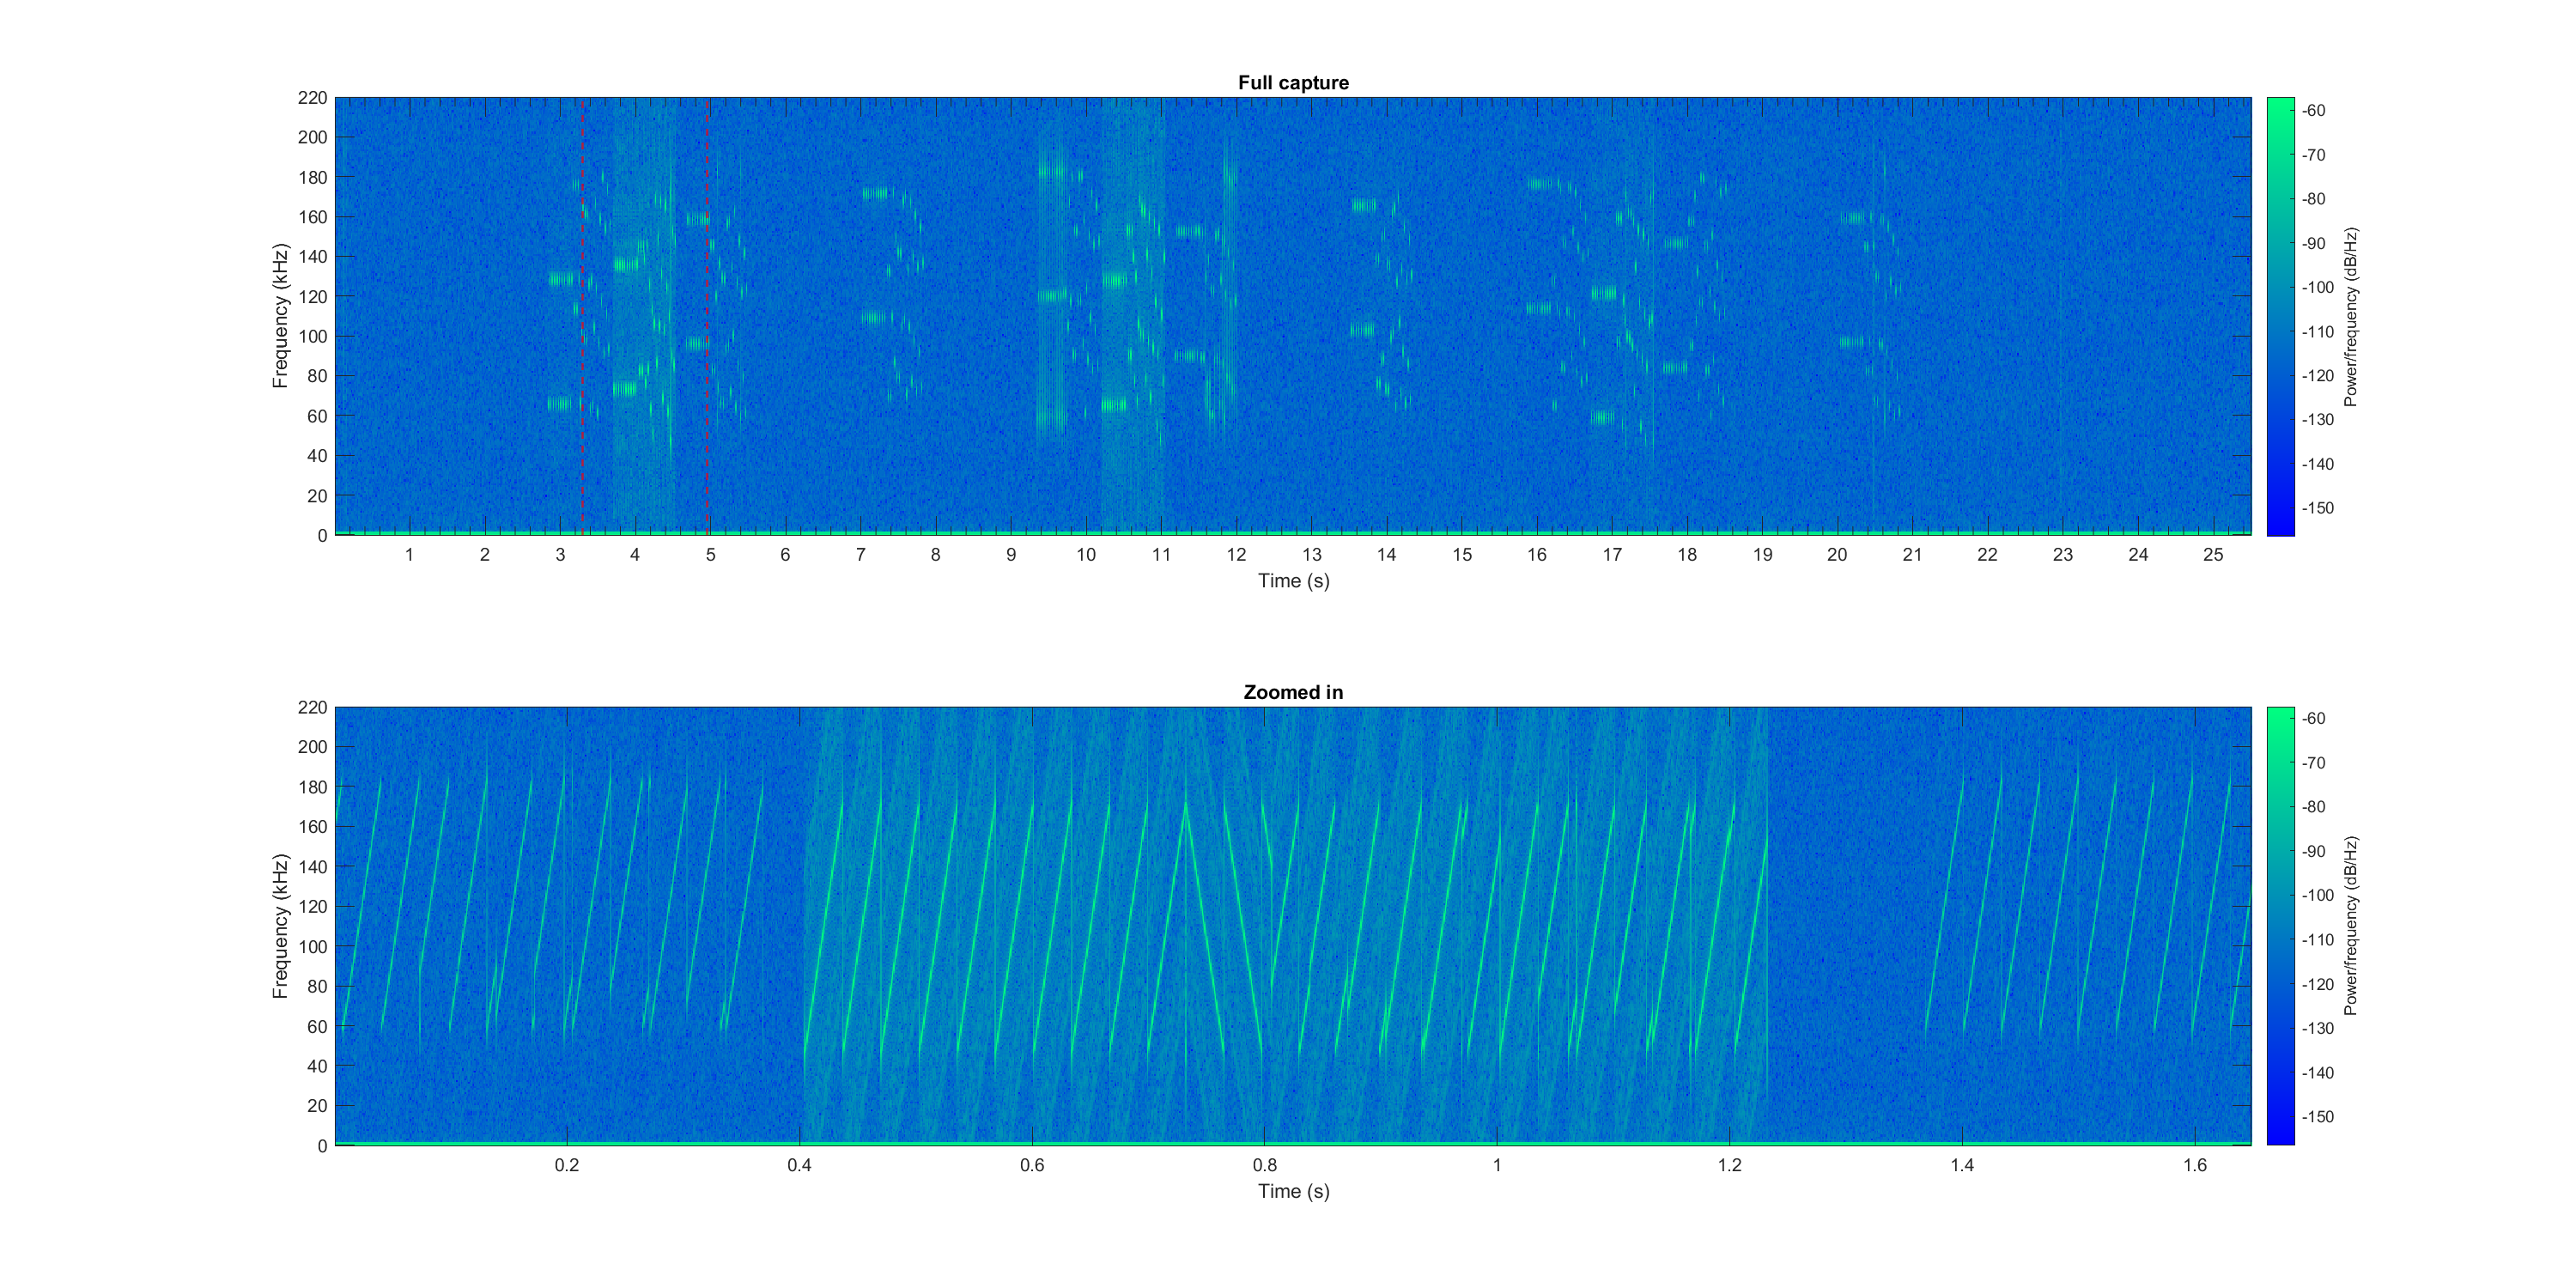
\includegraphics[width=\textwidth]{research/gqrx/zoom-win1024-sig1-lvl3}
    \caption{\label{img:signal1-level3}Spektrogram sygnałów z~pierwszej próbki wraz ze zbliżeniem między 3.4 s~a 5~s}
\end{figure}

\begin{figure}[!htbp]
    \centering
    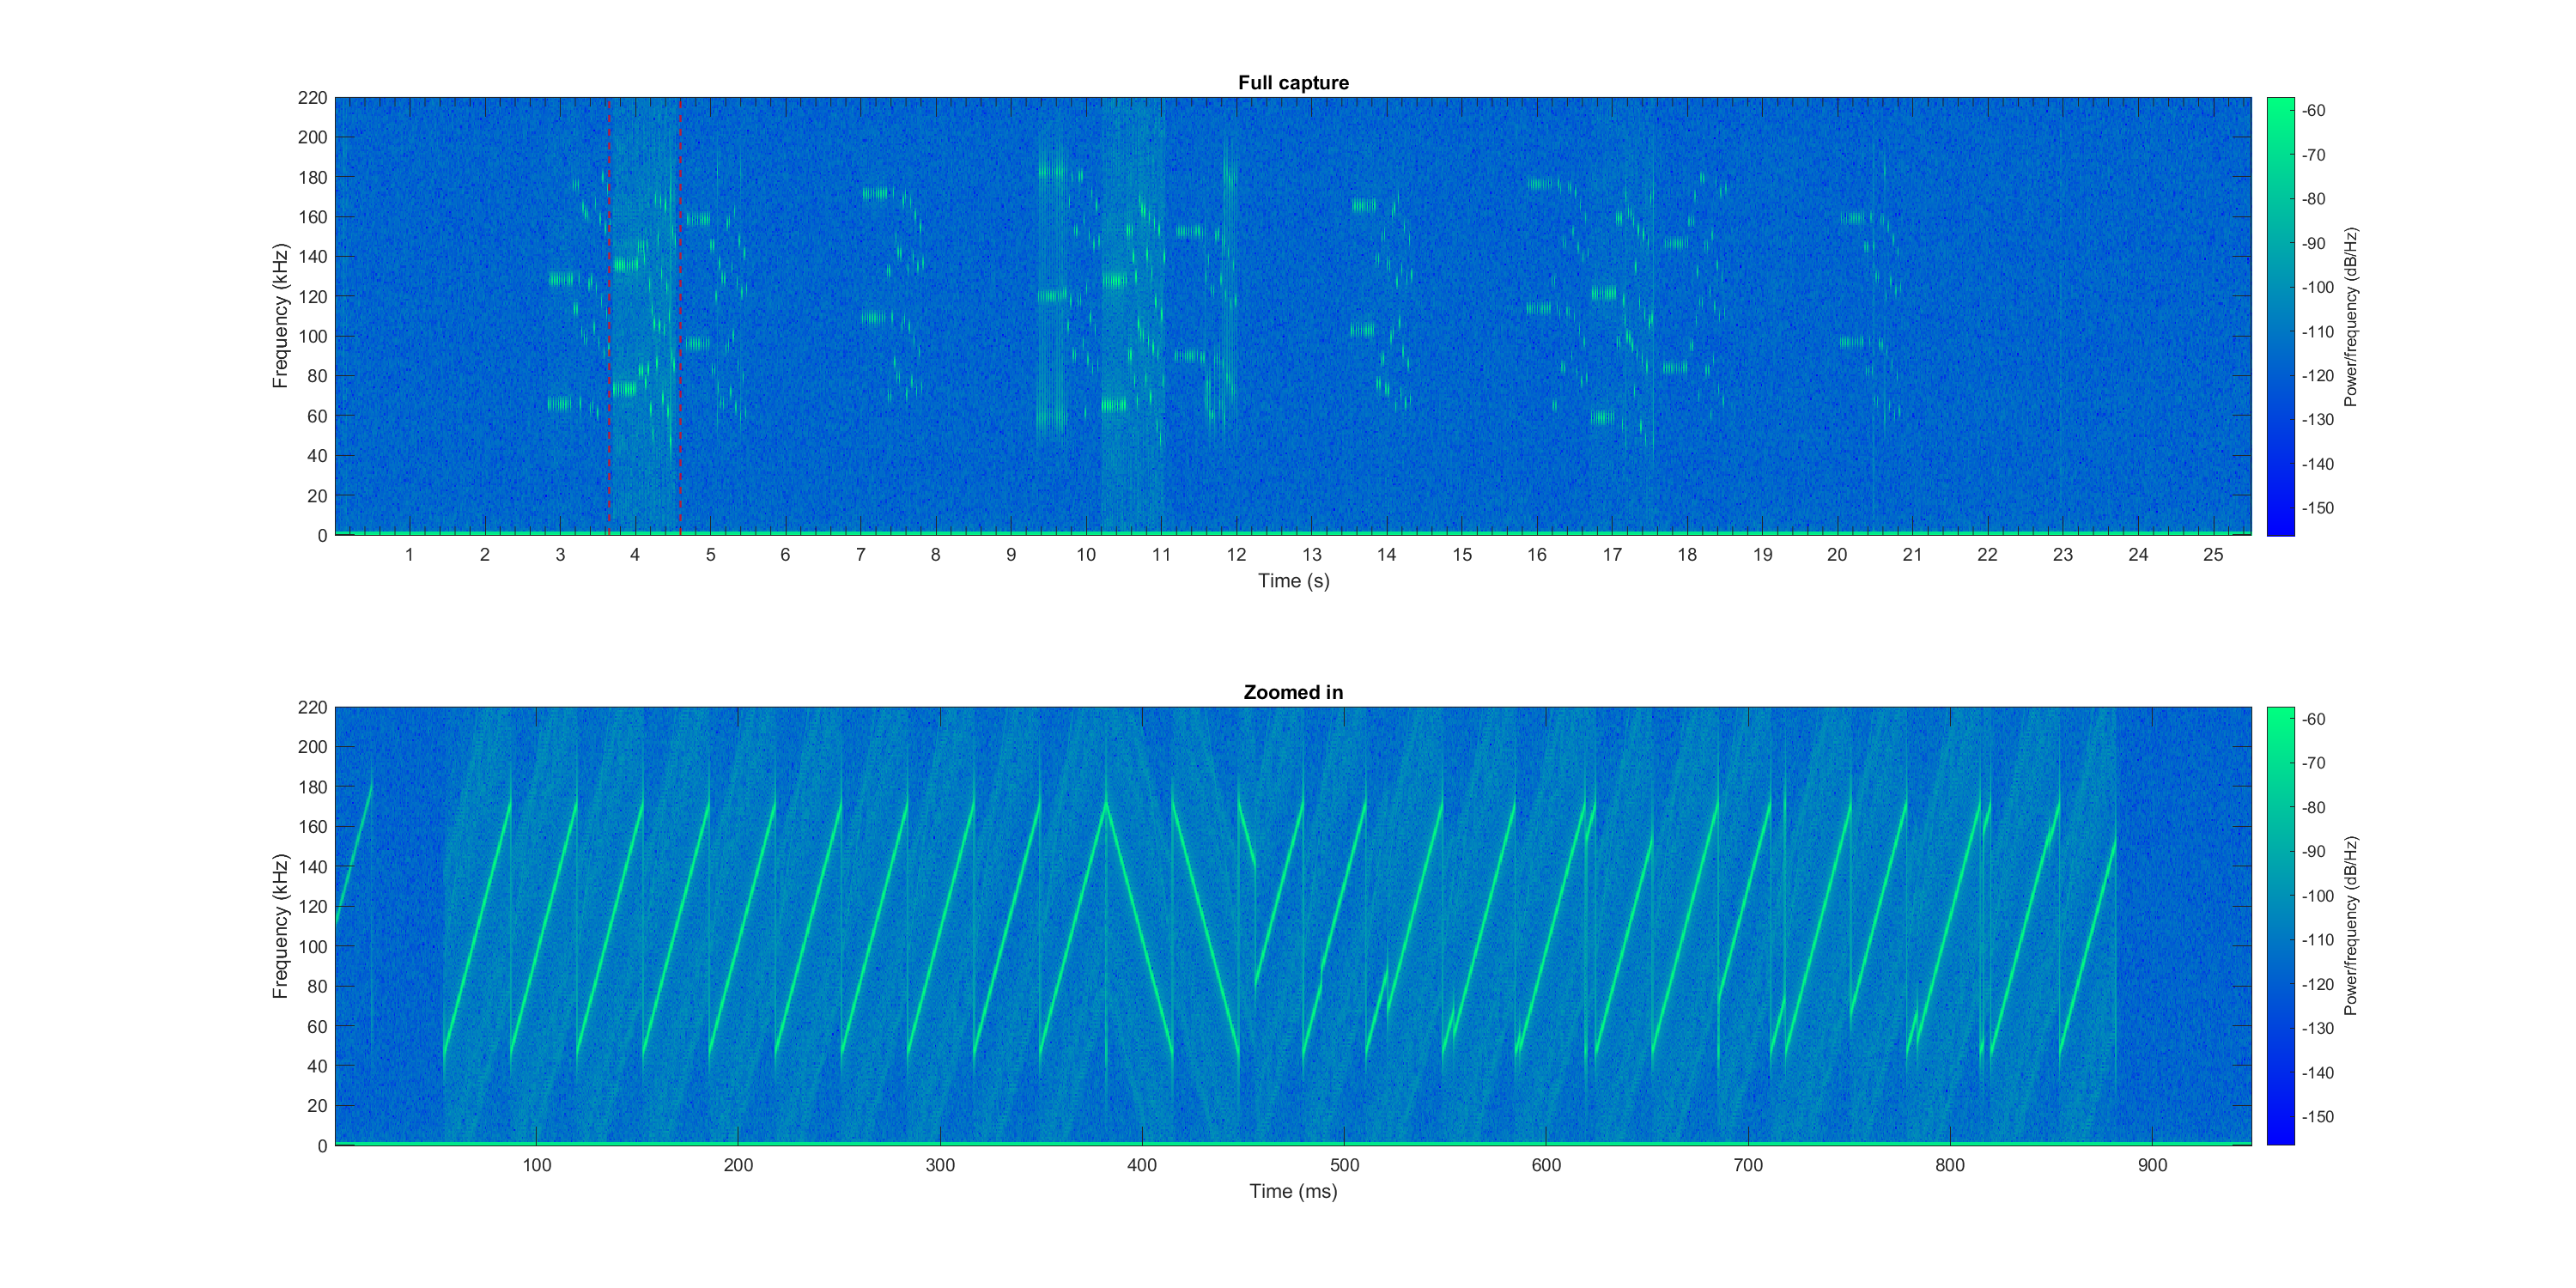
\includegraphics[width=\textwidth]{research/gqrx/zoom-win1024-sig1-lvl4}
    \caption{\label{img:signal1-level4}Spektrogram sygnałów z~pierwszej próbki wraz ze zbliżeniem między 3.6 s~a 4.6 s,
        widoczna jedna transmisja}
\end{figure}

\FloatBarrier
Na podstawie wygenerowanych spektrogramów możliwe było przeanalizowanie jednej pełnej ramki transmisji danych. Dzięki
uzyskanemu dużemu przybliżeniu na analizowany sygnał możliwe było wyznaczenie granic poszczególnych elementów ramki
LoRa. Przedstawione zostało to na rys. \ref{img:signal2-zoomed-analysis} oraz \ref{img:signal3-zoomed-analysis}
(odpowiednio dla fragmentu z~zarejestrowanych próbek drugiej oraz trzeciej).

\begin{figure}[!htbp]
    \centering
    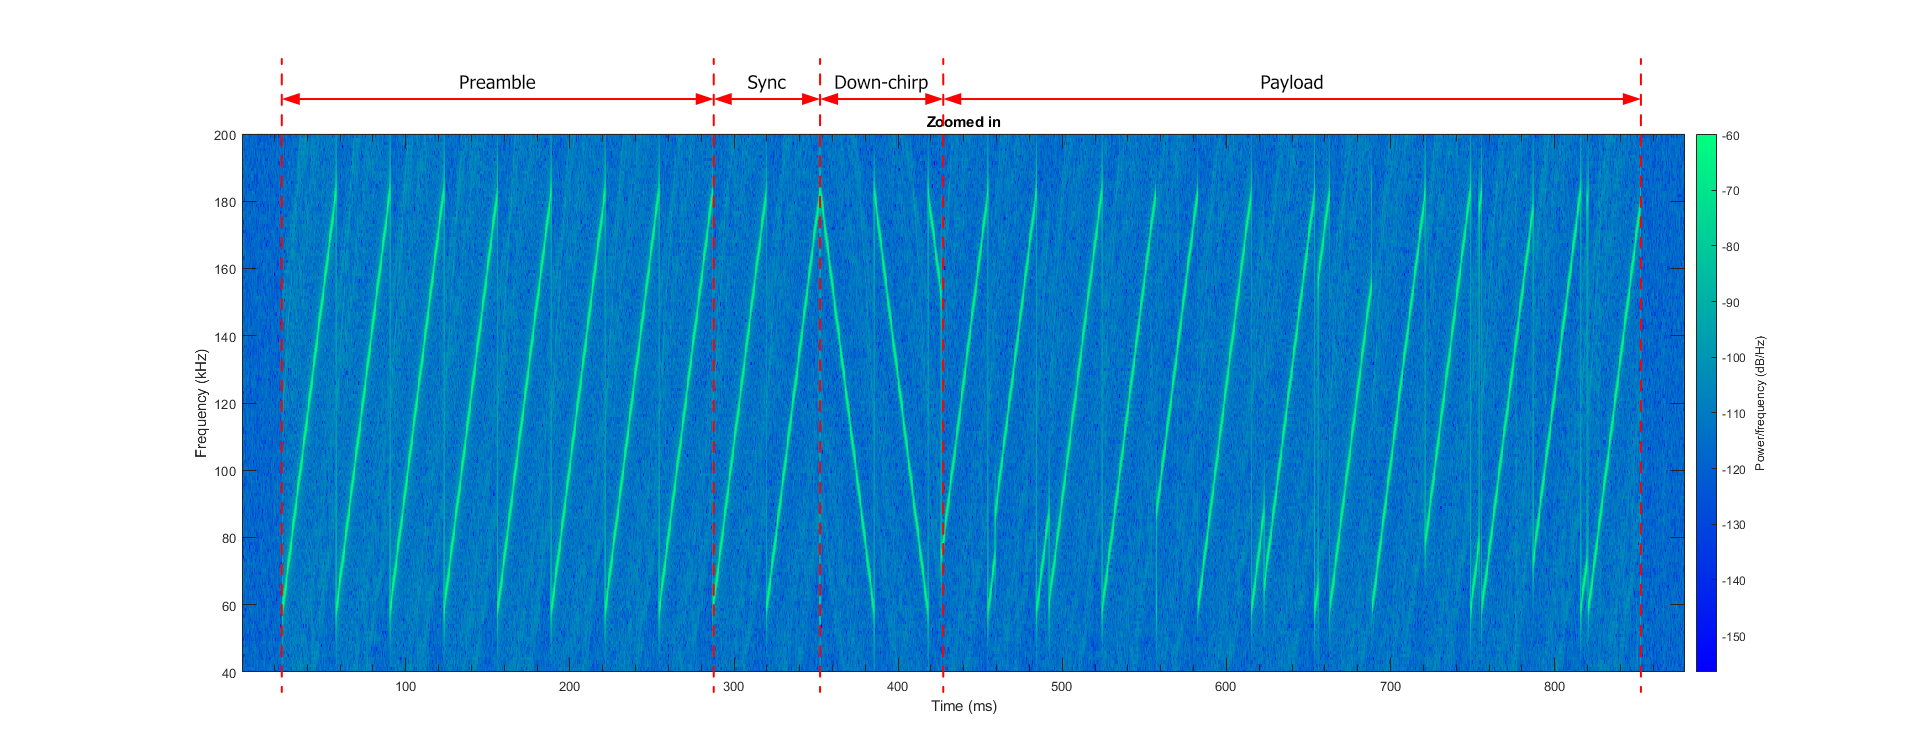
\includegraphics[width=\textwidth]{research/signal2-zoomed-analysis}
    \caption{\label{img:signal2-zoomed-analysis}Fragment drugiej próbki sygnału z~oznaczonymi poszczególnymi elementami
        ramki LoRa}
\end{figure}

\begin{figure}[!htbp]
    \centering
    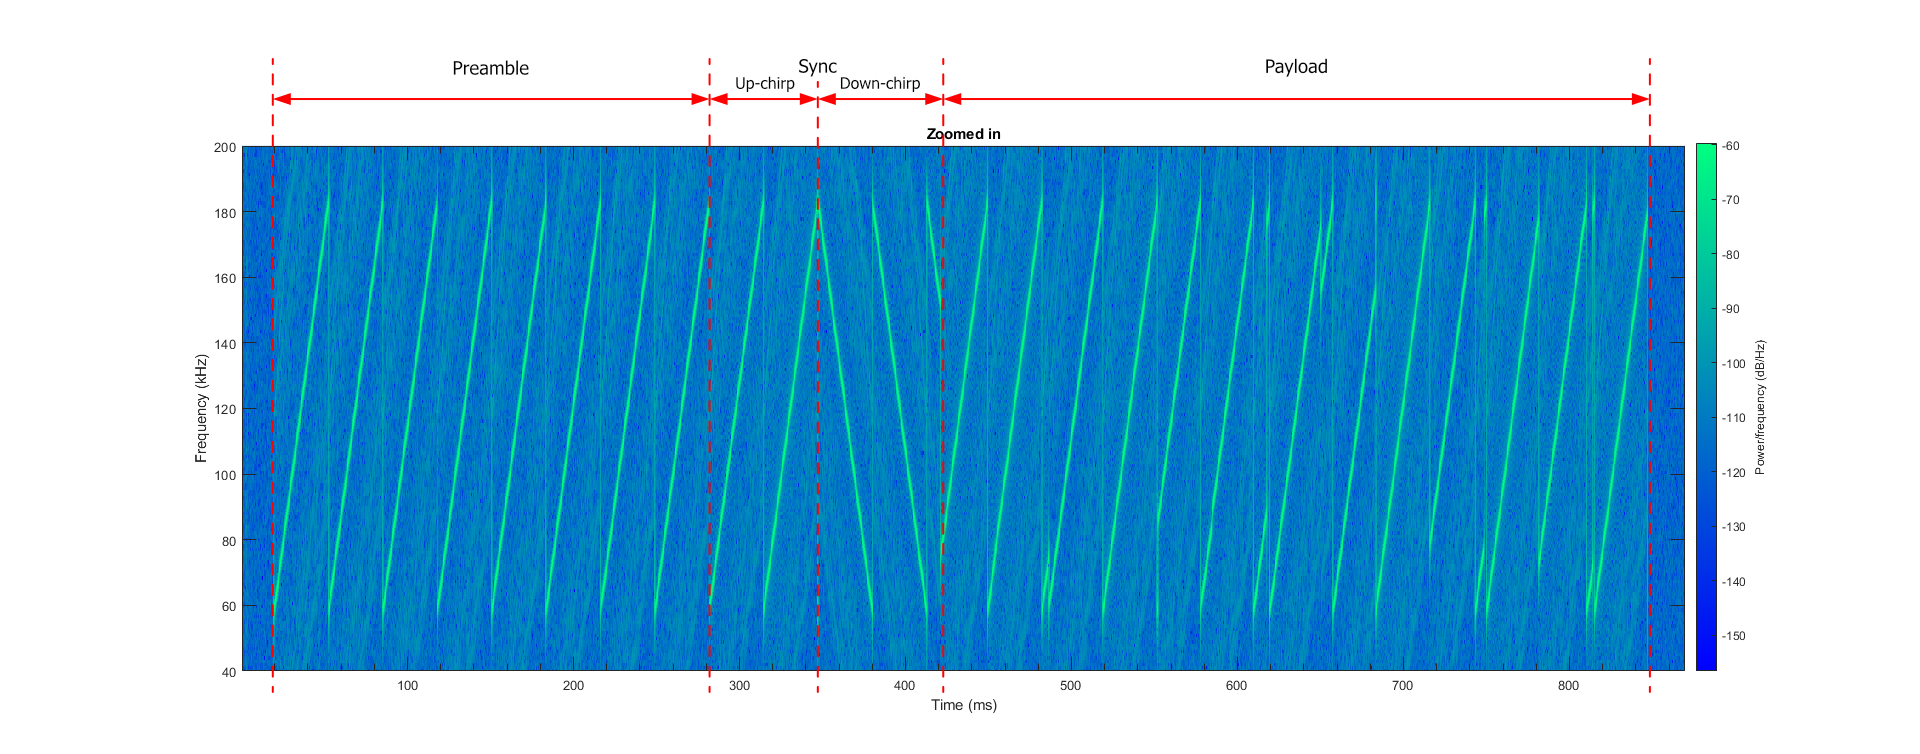
\includegraphics[width=\textwidth]{research/signal3-zoomed-analysis}
    \caption{\label{img:signal3-zoomed-analysis}Fragment trzeciej próbki sygnału z~oznaczonymi poszczególnymi elementami
        ramki LoRa}
\end{figure}

\FloatBarrier
Na przedstawionych fragmentach spektrogramów widoczne są różnice, pokazujące, że możliwe jest w~pewnym stopniu
rozróżnienie elementów transmisji. Są one widoczne tylko w~częściach oznaczonych jako "Payload" na wygenerowanych
wykresach, ponieważ tylko te elementy są zmienne w~każdej transmisji -- zawierają nagłówek, właściwe przesyłane dane
oraz kod CRC (ang. \textsl{Cyclic Redundancy Check}, służący wykrywaniu potencjalnych błędów w~transmisji). Pozostałe
elementy są elementami stałymi dla każdej ramki: preambuła (której długość ustawiona została na 8~symboli) -- pozwala
innym elementom sieci na wykrycie początku transmisji ramki, a~także dodatkowe symbole w~modulacjach Up-chirp (niższe do
wyższych częstotliwości) oraz Down-chirp (wyższe do niższych częstotliwości) -- w~sumie 4.25 symbolu, służące
synchronizacji, aby mieć jak największą pewność, że dane, które mają zostać przesłane, nie zostaną w~żaden sposób
zniekształcone przez ew. przesunięcia w~czasie.

Ponieważ każda ramka LoRa jest kodowana, możliwe jest jedynie rozróżnienia pojedynczych ramek między sobą, jednakże nie
jest już możliwe, korzystając wyłącznie ze spektrogramów, rozpoznanie co w~danym momencie jest przesyłane.
W~zaprezentowanych ramkach z~dwóch różnych próbek widać pewne różnice w~przesyłanych symbolach, jednakże tylko na
podstawie tego nie jest możliwe pokazanie, które symbole przedstawiają konkretne bity przesyłanych wiadomości.

\FloatBarrier

\section{\label{sect:network-communication-params}Badanie parametrów komunikacyjnych sieci} Kolejnym elementem wartym
zbadania w~przypadku budowania sieci bezprzewodowych jest określenie ich możliwości komunikacji. Parametry, jakie
zostały sprawdzone to skuteczny zasięg komunikacji oraz przepustowość sieci -- teoretycznie, korzystając z~dostępnych
wzorów, w~celu określenia co jest możliwe do uzyskania oraz porównanie faktycznie uzyskanymi wynikami, na podstawie
zebranych danych I/Q oraz wygenerowanych spektrogramów.

\subsection{\label{sect:network-communication-range}Skuteczny zasięg komunikacji} Zasięg komunikacji sprawdzony został
dla dwóch różnych przypadków. Modyfikując wartość parametru Spreading Factor (SF, długość symbolu, związana z~ilością
przesyłanych bitów) sprawdzone zostały dwa skrajne przypadki -- krótkie, szybkie transmisje dla SF7 oraz wolniejsze,
dłuższe transmisje dla SF12. Badanie przeprowadzone zostało w~terenie średnio zabudowanym i~częściowo zalesionym.
Otoczenie to wybrane zostało, ponieważ założyć można było, że komunikacja między modułami będzie odbywać się bez
zakłóceń zewnętrznych pochodzących z~innych urządzeń nadających na tym samym paśmie co badana sieć.

Według specyfikacji standardu oraz na podstawie innych badań teoretyczny zasięg komunikacji między modułami określony
został na 5~km \cite{lora-phy-range-test}. Podczas badania wykorzystane zostało nieznacznie zmodyfikowane oprogramowanie
-- wyłączona została funkcja zegara i~każdorazowo zapytania były wysyłane ręcznie, wykorzystując do tego przycisk na
module MASTER.

Scenariusz badania opierał się na pozostawieniu modułów SLAVE podłączonych do komputera stacjonarnego (w celu
późniejszej obserwacji logów z~ich pracy), natomiast modułem \enquote{poruszającym się} był moduł MASTER. Wykorzystując
dostępne online mapy, określone zostały miejsca, gdzie należało się zatrzymać i~zainicjować transmisję. Badanie nie
zostało wykonane w~ruchu, aby moduły miały jak największe szanse na uzyskanie połączenia, a~także dlatego, że celem
badania było symulowanie statycznej sieci operującej na dużych odległościach, a~nie mobilnego punktu pomiarowego.
Dodatkowo podczas badania sprawdzony został wpływ dość gęstego lasu na możliwości komunikacji modułów. Testy
przeprowadzone zostały zwiększając odległość od modułów SLAVE co około 100 m~za każdym razem.

Na podstawie uzyskanych wyników sporządzona została mapa (rys. \ref{img:distance-research-map}) przedstawiająca
odległości, które pozwoliły na uzyskanie komunikacji między modułami.

\begin{figure}[!htbp]
    \centering
    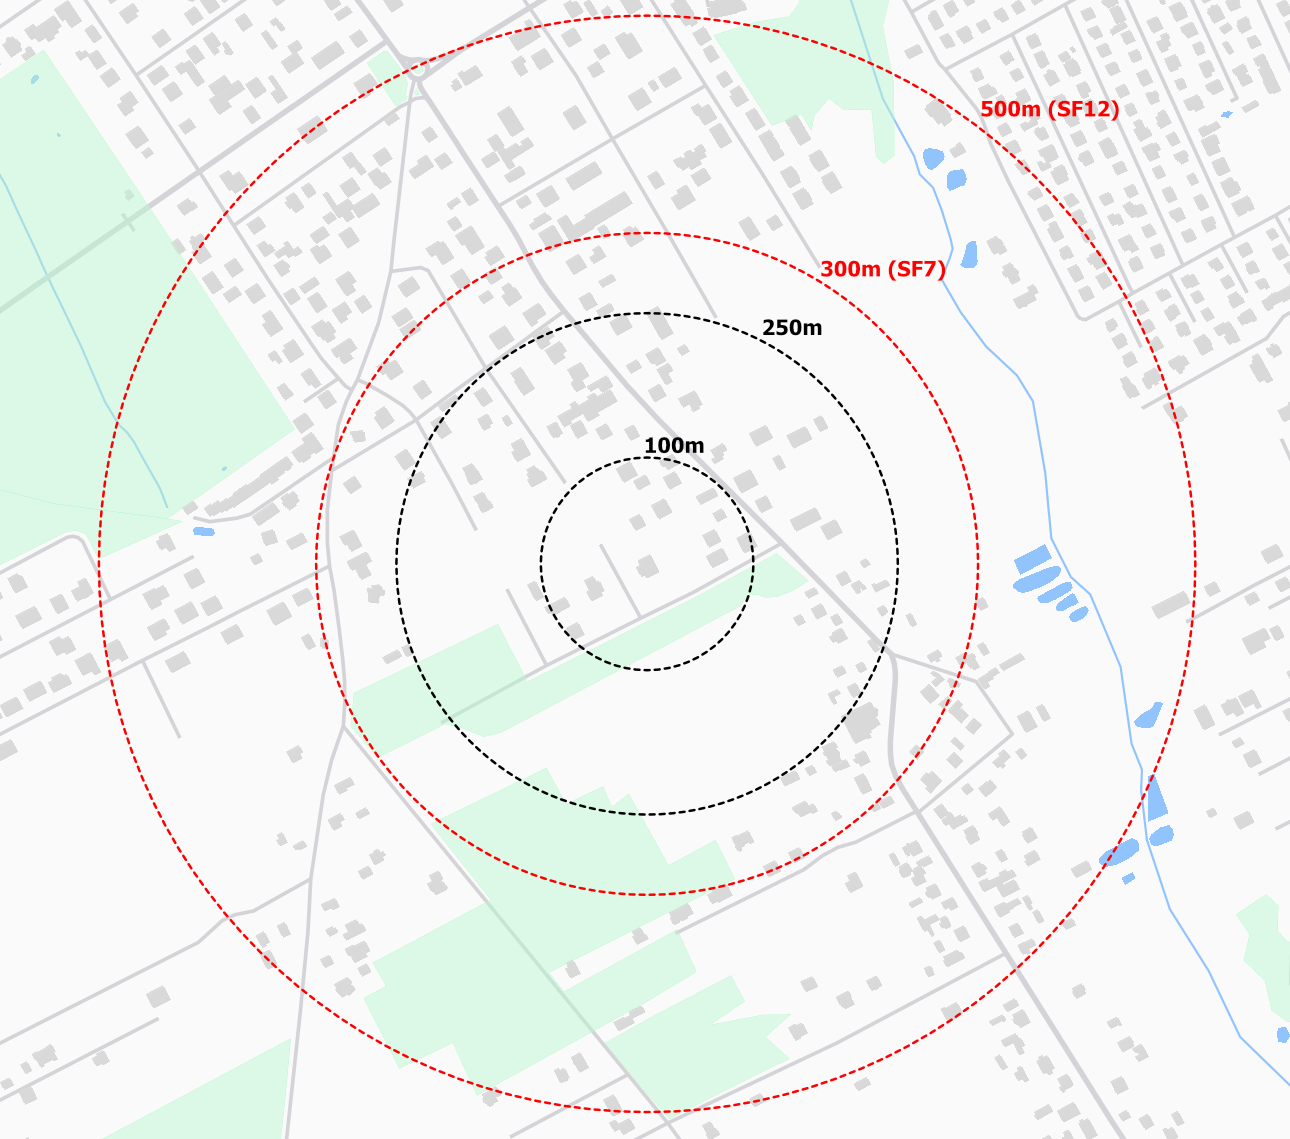
\includegraphics[width=0.9\textwidth]{research/distance-research-map}
    \caption{\label{img:distance-research-map}Mapa z~oznaczonymi odległościami, gdzie udało się uzyskać komunikację}
\end{figure}

\FloatBarrier
Wyniki uzyskane podczas badania były znacznie gorsze niż przedstawione w~innych pracach badających te możliwości
standardu LoRa. Kolorem czerwonym na mapie zaznaczone zostały odległości, które pozwoliły na uzyskanie jakiejkolwiek
komunikacji pomiędzy modułami dla ustawienia SF7 oraz SF12. W~obu przypadkach, w~odległościach większych niż zaznaczone,
każdorazowe wysłanie zapytania z~modułu MASTER kończyło się brakiem jakiejkolwiek odpowiedzi od modułów SLAVE.

Na podstawie uzyskanych wyników pojawia się wniosek, że aby możliwym było uzyskanie znacznie większych odległości
komunikacji między modułami, środowisko, w~jakim one pracują, musiałoby być znacznie mniej zabudowane oraz pozbawione
znacznej ilości przeszkód, jakie mogły występować podczas badania. Jednakże uzyskane wyniki pokazują też, że możliwe
jest zbudowanie oraz zaimplementowanie sieci, która pozwala na komunikację na znacznych dystansach.

\subsection{\label{sect:network-communication-bitrate}Badanie przepustowości sieci} Niezależnie od tego, czy budowana
jest sieć przewodowa, czy bezprzewodowa, ważnym parametrem jest jej przepustowość. W~przypadku, gdy będzie ona zbyt
niska, sieć mogłaby nie spełniać założeń projektowych lub wymagań, które zostały przyjęte. W~przypadku zaprojektowanej
oraz zaimplementowanej sieci czujnikowej parametr nie był kluczowy, pomimo tego został on zbadany, w~celu określenia
możliwości stworzonego rozwiązania.

Pierwszym elementem było określenie teoretycznych parametrów, które sieć powinna móc osiągnąć dla obu skrajnych
przypadków -- SF7 oraz SF12. Następnie, korzystając z~otrzymanej analizy danych I/Q podjęta została próba porównania
otrzymanych wyników do wyliczonych wartości teoretycznych.

Parametrami, które brane są pod uwagę przy określaniu przepustowości sieci LoRa, są:
\begin{itemize}[label=--]
    \item Spreading Factor, $\mathit{SF}$, określa ilość bitów na symbol,
    \item Code Rate, $\mathit{CR}$, używany do określenia stosunku bitów użytecznych do ilości bitów przesyłanych,
    \item Bandwidth, $\mathit{BW}$, szerokość pasma transmisji.
\end{itemize}
Do wyznaczenia wartości teoretycznych przyjęte zostały $\mathit{CR}$ = 1~oraz $\mathit{BW}$ = 125 kHz, ponieważ dla
takich ustawień zebrane zostały dane I/Q podczas analizy widmowej sygnałów.

Do określenia nominalnej, teoretycznej przepustowości $\mathit{Rb}$ wykorzystana została zależność przedstawiona
równaniem \ref{eqn:lora-bitrate}:
\begin{equation}\label{eqn:lora-bitrate}
    \mathit{Rb} = \mathit{SF}\cdot\cfrac{4\cdot{(4+\mathit{CR})^{-1}}}{2^{\mathit{SF}}\cdot{\mathit{BW}^{-1}}}\cdot{1000}\quad\text{[bps]}
\end{equation}

Dla ustawienia Spreading Factor, SF7 (7 bitów na symbol) nominalna przepustowość sieci równa jest:
\begin{equation*}
    \mathit{Rb} = \mathit{SF}\cdot\cfrac{4\cdot{(4+\mathit{CR})^{-1}}}{2^{\mathit{SF}}\cdot{\mathit{BW}^{-1}}}\cdot{1000} = 7 \cdot \frac{4 \cdot 5^{-1}}{2^7\cdot 125^{-1}} \cdot 1000 = 5468.75\,\text{bps} = 5.47\,\text{kbps}
\end{equation*}
natomiast dla SF12 (12 bitów na symbol) wartość ta jest znacznie mniejsza:
\begin{equation*}
    \mathit{Rb} = \mathit{SF}\cdot\cfrac{4\cdot{(4+\mathit{CR})^{-1}}}{2^{\mathit{SF}}\cdot{\mathit{BW}^{-1}}}\cdot{1000} = 12 \cdot \frac{4 \cdot 5^{-1}}{2^{12}\cdot 125^{-1}} \cdot 1000 = 293\,\text{bps}
\end{equation*}

Korzystając ze spektrogramów wygenerowanych na podstawie danych I/Q, przedstawionych na rys.
\ref{img:signal2-zoomed-analysis} oraz \ref{img:signal3-zoomed-analysis} możliwe było określenie, że na każdą
z~zarejestrowanych transmisji składało się w~sumie 24 do 25 symboli (8 preambuły, 4.25 synchronizacji oraz około 12
właściwej przesyłanej wiadomości), które zostały przesłane w~czasie około 820 milisekund. Wiedząc, że zarejestrowane
transmisje korzystały z~ustawienia SF12 (czyli 12 bitów na symbol), wyznaczona została ilość przesłanych w~sumie bitów
-- około 290. Na podstawie tych informacji możliwe było określenie szacowanej uzyskanej szybkości transmisji
(przepustowości sieci) na około 353 bps (bitów na sekundę). Otrzymane wartości były zbliżone do wartości nominalnych,
w~tym przypadku nawet wyższe niż zostało to wyznaczone teoretycznie.

\FloatBarrier
\section{\label{sect:network-power-params}Badanie poboru prądu i~zużycia energii} Ważnym elementem określającym jak
dobrze może działać sieć bezprzewodowa, jest jej zużycie energii oraz możliwość pracy tylko na zasilaniu bateryjnym.
W~tym celu zbadano pobór prądu modułów w~różnych momentach:
\begin{itemize}[label=--]
    \item praca normalna (stan \enquote{IDLE}, spoczynku, aktywny tylko zegar),
    \item aktywna komunikacja między modułami,
    \item wykonywanie pomiarów otoczenia (moduły SLAVE),
    \item transmisja danych przez I2C (moduł MASTER).
\end{itemize}

Badanie wykorzystywało standardowe stanowisko testowe -- moduły SLAVE umieszczone w~odległości około 45 cm (0.45 m) od
modułu MASTER, gdzie wszystkie pracowały na niezmodyfikowanym oprogramowaniu. Testy nie obejmowały sprawdzenia poboru
prądu przez moduł serwera sieciowego z~uwagi na to, że nie posiadał dostępnego miejsca pomiarowego, a~pomiary
z~wykorzystaniem jego portu USB posiadałyby znaczną niedokładność pomiarową powiązaną przykładowo z~poborem prądu innych
elementów płytki (np. diod LED). Na podstawie zebranych danych wyznaczone zostały pobór mocy przez moduły oraz
teoretyczny maksymalny czas pracy na zasilaniu bateryjnym.

\subsection{\label{sect:network-modules-current-draw}Badanie poboru prądu przez moduły sieci} Wykorzystane moduły STM32
L152 Nucleo-64 wyposażone są w~zworkę JP6 umieszczoną za stabilizatorem napięcia, z~której był zasilany mikrokontroler
STM32L152RE. Fragment schematu z~dokumentacji płytki \cite{stm-product-overview} z~oznaczoną zworką przedstawiony został
na rys. \ref{img:stm32-l152re-schematic-frag}. Gdy była ona założona na wyprowadzone piny, mikrokontroler był zasilany,
wykorzystując płytkę rozszerzenia ze złączem Mini USB typu B, z~portu USB komputera, gdzie moduł był podłączony.
W~momencie, gdy była ona usunięta, możliwe było w~to miejsce podłączenie amperomierza, co umożliwiało pomiar prądu
pobieranego bezpośrednio przez mikrokontroler.

\begin{figure}[!htbp]
    \centering
    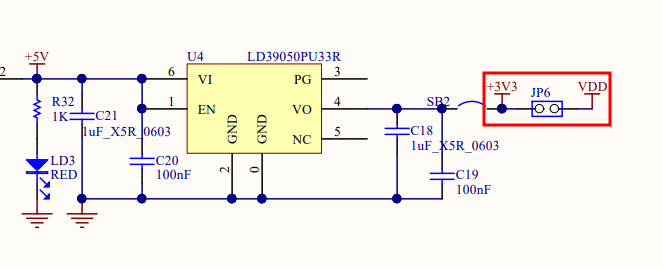
\includegraphics[width=0.7\textwidth]{screenshots/stm32-l152re-schematic-frag}
    \caption{\label{img:stm32-l152re-schematic-frag}Fragment schematu płytki wykorzystanego modułu STM32 Nucleo-64.
        Napięcie VDD wyprowadzone jest bezpośrednio do zasilania mikrokontrolera}
\end{figure}

\FloatBarrier

Wykorzystując monitor portu szeregowego, gdzie logowane są informacje o~pracy modułów oraz opisaną metodę pomiaru
pobieranego prądu zebrane zostały jego wartości w~wyszczególnionych momentach pracy. Ponieważ pobór nie był równomierny
przez cały czas pracy modułów, szczególnie w~przypadkach aktywnej komunikacji oraz pracy w~stanie IDLE, w~tych momentach
zebrano szereg pomiaru, a~następnie wyznaczona została ich średnia. Otrzymane wyniki zebrane zostały w~tabelach
\ref{tab:power-usage-sf7a}, \ref{tab:power-usage-sf7b} oraz \ref{tab:power-usage-sf12a}, \ref{tab:power-usage-sf12b},
odpowiednio dla ustawień SF7 oraz SF12.

\renewcommand\theContinuedFloat{\alph{ContinuedFloat}}
\begin{table}[!htbp]
    \ContinuedFloat*
    \centering
    \caption{\label{tab:power-usage-sf7a}Wyniki pomiarów poboru prąd przez moduły MASTER, SLAVE 1 dla SF7.}
    \begin{tabular}{ccccccc}
        \toprule
        \multicolumn{1}{c}{\multirow{2}[4]{*}{Tryb pracy}} & \multicolumn{3}{c}{MASTER} & \multicolumn{3}{c}{SLAVE 1}                                                                                                             \\
        \cmidrule{2-7}                                     & \multicolumn{1}{c}{Min.}   & \multicolumn{1}{c}{Typ.}    & \multicolumn{1}{c}{Max.} & \multicolumn{1}{c}{Min.} & \multicolumn{1}{c}{Typ.} & \multicolumn{1}{c}{Max.} \\
        \midrule
        Normalna, spoczynek [mA]                           & 11.21                      & 11.40                       & 11.55                    & 11.09                    & 11.14                    & 11.19                    \\
        \midrule
        Aktywna komunikacja [mA]                           & 11.69                      & 11.89                       & 12.12                    & 11.63                    & 11.77                    & 11.91                    \\
        \midrule
        Pomiary otoczenia [mA]                             & \multicolumn{3}{c}{nd.}    & 11.19                       & 11.28                    & 11.37                                                                          \\
        \midrule
        Transmisja po I2C [mA]                             & -                          & 11.60                       & -                        & \multicolumn{3}{c}{nd.}                                                        \\
        \bottomrule
    \end{tabular}%
\end{table}%

\begin{table}[!htbp]
    \ContinuedFloat
    \centering
    \caption{\label{tab:power-usage-sf7b}Wyniki pomiarów poboru prąd przez moduły SLAVE 2, SLAVE 3 dla SF7.}
    \begin{tabular}{ccccccc}
        \toprule
        \multicolumn{1}{c}{\multirow{2}[4]{*}{Tryb pracy}} & \multicolumn{3}{c}{SLAVE 2} & \multicolumn{3}{c}{SLAVE 3}                                                                                                             \\
        \cmidrule{2-7}                                     & \multicolumn{1}{c}{Min.}    & \multicolumn{1}{c}{Typ.}    & \multicolumn{1}{c}{Max.} & \multicolumn{1}{c}{Min.} & \multicolumn{1}{c}{Typ.} & \multicolumn{1}{c}{Max.} \\
        \midrule
        Normalna, spoczynek [mA]                           & 11.08                       & 11.12                       & 11.16                    & 11.46                    & 11.52                    & 11.58                    \\
        \midrule
        Aktywna komunikacja [mA]                           & 11.54                       & 11.61                       & 11.68                    & 11.88                    & 11.96                    & 12.04                    \\
        \midrule
        Pomiary otoczenia [mA]                             & 11.23                       & 11.28                       & 11.33                    & 11.25                    & 11.31                    & 11.37                    \\
        \midrule
        Transmisja po I2C [mA]                             & \multicolumn{3}{c}{nd.}     & \multicolumn{3}{c}{nd.}                                                                                                                 \\
        \bottomrule
    \end{tabular}%
\end{table}
\renewcommand\theContinuedFloat{\alph{ContinuedFloat}}
\begin{table}[!htbp]
    \ContinuedFloat*
    \centering
    \caption{\label{tab:power-usage-sf12a}Wyniki pomiarów poboru prąd przez moduły MASTER, SLAVE 1 dla SF12.}
    \begin{tabular}{ccccccc}
        \toprule
        \multicolumn{1}{c}{\multirow{2}[4]{*}{Tryb pracy}} & \multicolumn{3}{c}{MASTER} & \multicolumn{3}{c}{SLAVE 1}                                                                                                             \\
        \cmidrule{2-7}                                     & \multicolumn{1}{c}{Min.}   & \multicolumn{1}{c}{Typ.}    & \multicolumn{1}{c}{Max.} & \multicolumn{1}{c}{Min.} & \multicolumn{1}{c}{Typ.} & \multicolumn{1}{c}{Max.} \\
        \midrule
        Normalna, spoczynek [mA]                           & 11.12                      & 11.35                       & 11.52                    & 11.13                    & 11.23                    & 11.25                    \\
        \midrule
        Aktywna komunikacja [mA]                           & 11.69                      & 11.82                       & 12.12                    & 11.66                    & 11.84                    & 11.97                    \\
        \midrule
        Pomiary otoczenia [mA]                             & \multicolumn{3}{c}{nd.}    & 11.24                       & 11.37                    & 11.40                                                                          \\
        \midrule
        Transmisja po I2C [mA]                             & -                          & 11.71                       & -                        & \multicolumn{3}{c}{nd.}                                                        \\
        \bottomrule
    \end{tabular}%
\end{table}%

\begin{table}[!htbp]
    \ContinuedFloat
    \centering
    \caption{\label{tab:power-usage-sf12b}Wyniki pomiarów poboru prąd przez moduły SLAVE 2, SLAVE 3 dla SF12.}
    \begin{tabular}{ccccccc}
        \toprule
        \multicolumn{1}{c}{\multirow{2}[4]{*}{Tryb pracy}} & \multicolumn{3}{c}{SLAVE 2} & \multicolumn{3}{c}{SLAVE 3}                                                                                                             \\
        \cmidrule{2-7}                                     & \multicolumn{1}{c}{Min.}    & \multicolumn{1}{c}{Typ.}    & \multicolumn{1}{c}{Max.} & \multicolumn{1}{c}{Min.} & \multicolumn{1}{c}{Typ.} & \multicolumn{1}{c}{Max.} \\
        \midrule
        Normalna, spoczynek [mA]                           & 11.22                       & 11.31                       & 11.37                    & 11.32                    & 11.38                    & 11.54                    \\
        \midrule
        Aktywna komunikacja [mA]                           & 11.68                       & 11.70                       & 11.81                    & 11.74                    & 11.86                    & 12.00                    \\
        \midrule
        Pomiary otoczenia [mA]                             & 11.33                       & 11.38                       & 11.48                    & 11.09                    & 11.15                    & 11.22                    \\
        \midrule
        Transmisja po I2C [mA]                             & \multicolumn{3}{c}{nd.}     & \multicolumn{3}{c}{nd.}                                                                                                                 \\
        \bottomrule
    \end{tabular}%
\end{table}

\FloatBarrier
W~uzyskanych wynikach można zauważyć, że poszczególne momenty pracy modułów charakteryzują się różnymi wartościami
poboru prądu, a~zdecydowanie najwięcej wymagane było podczas komunikacji w~sieci.

Biorąc pod uwagę fakt, że zmiana parametru Spreading Factor w~przypadku zasięgu komunikacji wprowadziła znaczącą zmianę
w~możliwościach komunikacji, złożone zostało, że podobne zachowanie zostanie zaobserwowane w~przypadku poboru prądu --
moduły przez wydłużony czas komunikacji będą pobierały widocznie więcej prądu. Jednakże w~przypadku tego badania takie
zachowanie nie zostało zaobserwowane. Moduły pobierały bardzo zbliżony prąd niezależnie od ustawienia, a~różnice
w~otrzymanych wartościach można przypisać do niedokładności pomiarowej, różnic w~elementach aktywnych oraz pasywnych
wykorzystanych do produkcji, a~także do nieznacznych różnic w~samych mikrokontrolerach na użytych płytkach.

\subsection{\label{sect:network-work-on-battery}Maksymalny teoretyczny czas pracy sieci} Na podstawie uzyskanych wyników
pomiarów wyznaczone zostały średnie wartości poboru prądu dla każdego z~modułów. Z~uwagi na to, że nie zaobserwowano
znaczących różnic między ustawieniami SF7 oraz SF12, obliczenia wykonane zostały tylko dla przypadku SF7:
\begin{itemize}[label=--]
    \item moduł MASTER: 11.63 mA,
    \item moduł SLAVE 1: 11.39 mA,
    \item moduł SLAVE 2: 11.34 mA,
    \item moduł SLAVE 3: 11.73 mA.
\end{itemize}
Na podstawie otrzymanych wartości zauważyć można, że moduł SLAVE 3~charakteryzował się największym średnim poborem prądu
spośród wykorzystanych modułów.

Do wyznaczenia teoretycznego maksymalnego czasu pracy modułów na zasilaniu bateryjnym przyjęta została pojemność takiego
zasobnika na 10000 mAh -- wartość taka jest często spotykana w~dostępnych na rynku powerbankach (zasilaniach
bateryjnych stosowanych np. do telefonów), które mogą zasilać urządzenia poprzez podłączenie ich przez USB. Do obliczeń
wykorzystana została zależność przedstawiona równaniem \ref{eqn:battery-life}:

\begin{equation}\label{eqn:battery-life}
    \textsl{Żywotność baterii} = \frac{\textsl{Pojemność baterii (mAh)}}{\textsl{Prąd obciążenia (mA)}}\quad\text{[h]}
\end{equation}

Obliczenia wykonane zostały dla przypadku największego poboru prądu przez moduły (SLAVE 3), zakładając ciągłą,
nieprzerwaną pracę modułu. Otrzymana została wartość:
\begin{equation*}
    \textsl{Żywotność baterii} = \mathsf{\frac{10000}{11.73}} = \mathsf{852.5}\,\text{h}
\end{equation*}
co przeliczając, równa się 35.52 dniom (lub niespełna 5~tygodniom). Biorąc pod uwagę możliwie większe zużycie energii
związane z~zasilaniem także innych elementów wykorzystanych płytek (diody LED, czujniki BME280, itp.) wartość ta byłaby
w~pewnym stopniu mniejsza. Otrzymane wyniki pokazują, że sieć bazująca na standardzie LoRa mogłaby zostać wykorzystana
do zbudowania sieci czujnikowej, która wymagałaby niewielkiego wkładu pracy w~jej utrzymanie.